% !TeX root = ./main.tex

% ------------------------------------------------------------------------------------

\chapter[INTRODUCTION]{INTRODUCTION}

% Very general introduction why the topic of the thesis is relevant.

% Road Safety Scenario in the World and in Brazil.

% Urban planning having a crucial role on the road safety in cities.

\section{OBJECTIVES}

In the context of the urban planning practices and road safety management, the main objective of this research is to investigate the influence of demographic, socioeconomic, land use and constructed environment on the speeding practices as a risk factor on the frequency and severity of road crashes. The scenario of the study is the city of Curitiba, capital of the state of Paraná, Brazil. The correlation will be analyzed with the use of the Geographically Weighted Regression statistical model.

With the use of speeding data collected from drivers that participated in a Naturalistic Driving Study (NDS) performed in Curitiba, this investigation aims to contribute to the knowledge of its relationship with variables from the built environment (BE). These BE variables are categorized by \textcite{Ewing2009} in five groups called '5D': density, diversity, design, destination accessibility and distance to transit. In addition to these variables, this study aims to relate the income as a socioeconomic variable to the speeding as well.

As co-benefits in the investigation, this thesis aims to offer some level of insight regarding the development and update of speed control in cities, considering the operational and structural planning guidelines for the road systems and land use. With these factors in mind, it could be possible to present new ideas to the planning practices in Curitiba, regarding mobility plans, master plans and zoning laws.
    

\section{JUSTIFICATION}

The excess of traffic speed performed by vehicles on urban environments are a main risk factor in the chance and severity of road crashes, considering there is great volume of interaction between motorized and vulnerable users \cite{Elvik2009}. Considering the direct relationship between the mobility, the land use patterns and the built environment \cite{DeVos2013}, it is important to investigate these factors in search of improvements in the management process of the road safety. Speeding, which is on the primary causes for traffic crashes \cite{WHO2013} can be better studied and analyzed by the collection of naturalistic data.

Having in mind that most of the traffic crashes and conflicts happens in cities \cite{WHO2018}, as a consequence of the fast process of urbanization in the last decades, it is crucial to create safer conditions in these localities. In Brazil, the management of the mobility is attributed to the municipalities \cite{Brasil1997}. Therefore, the management of road safety, as a task inherent to traffic management, is also an attribution of the municipalities. It is necessary to observe the issues of road safety in cities when conducting the process of urban planning. Having this in mind, it was established laws in which this integration between the planning process by the municipalities and the sustainable mobility are clearly defined: The Statute of the Cities \cite{Brasil2001} and The Law of the Urban Mobility \cite{Brasil2012}.    

The built environment can affect the traffic safety through three main mediators: the traffic volumes, traffic conflicts and traffic speeds - which can directly affect the crash safety and severity in urban environments \cite{Ewing2009}. Traffic crashes are a final outcome of the problems involving the road safety. Therefore, in order to have a method to analyzed the operational conditions of the traffic safety in cities, it can be beneficial to use a intermediate outcome - or a safety performance indicator (SPI) \cite{Bastos2014} - which can be the amount of speeding that occurs across its territory, in addition to the studies that uses the traffic crashes as dependent variables. 

\section{THESIS STRUCTURE}

%% General composition of the thesis, giving which chapters the reader should expect

%% Write this part after completion of chapters 2 and 3

% ------------------------------------------------------------------------------------

\chapter{LITERATURE REVIEW}

This Chapter is divided into 5 sections, each presenting a relevant subject to the study. Section \ref{sec:rss} has discussions involving the road safety problems that occurs and how they can be managed. Section \ref{speeding} presents the main risk factor investigated in this document: speeding. It is discussed how it is related to the road safety, the factors that can influence speeding and how its occurrence can be investigated. Section \ref{be} includes the discussion about the built environment and it's variables, relating to the road safety performance and urban planning practices. Section \ref{nds} discusses naturalistic driving studies as a method of speeding data collection, and how it was performed in previous works. Section \ref{sec:gwr} discusses about the geographically weighted regression statistical method, and how it can be used to investigate built environment variables and road safety outcomes.

\section{ROAD SAFETY SCENARIO} \label{sec:rss}

Road traffic crashes around the world claims more than 1.3 million lives in each year, representing the eighth leading cause of deaths and causing up to 50 million injuries. Low and middle income countries (LMICs), including Brazil, suffers from traffic crashes death rates three times higher when compared to developed countries \cite{WHO2018}. The increasing number of traffic crashes deaths on LMICs is a consequence of a intense process of motorization that has been occurring in the last decades. To \textcite{Bhalla2016}, it is important to understand the evolution of road safety management on OECD developed countries in order to overcome the road safety problems in LMICs. 

Over the last century, the road safety performance of the OECD countries showed a consistent pattern. The road traffic death rate (per 100,000 population) in these countries were rising until the 1960s, as seen in \autoref{fig:oecd}. After this period, all countries showed a declining pattern, whilst the LMICs still had a rising pattern due to the rapid growth in their motor vehicle fleets. This behavior of rising and declining trend on the road traffic death rate could be explained by three phenomenons: economic determinism, risk substitution and a political shift in the road safety paradigm \cite{Bhalla2016}.

\begin{figure}[!htbp]
    \centering\footnotesize
    \captionsetup{font=footnotesize}
    \caption{ROAD TRAFFIC RATES IN OECD COUNTRIES}
    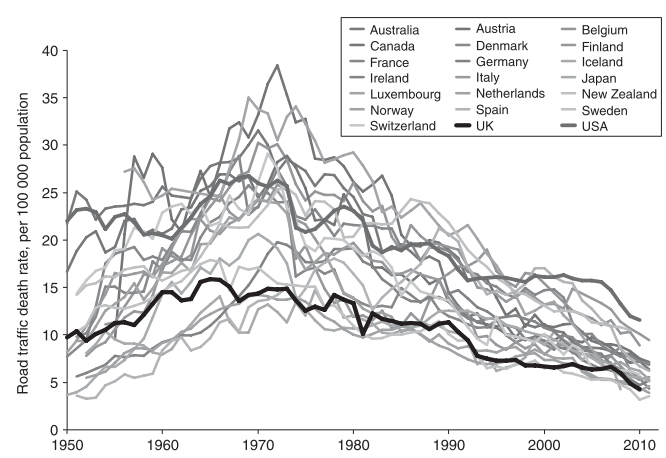
\includegraphics[width=0.8\textwidth]{fig/oecd.png}
    \label{fig:oecd}
    \par SOURCE: \textcite{Bhalla2016}.
\end{figure}

In the scope of economic determinism, the road traffic deaths are defined as a process related to the country development. The rising pattern is associated with the increase in motorization, and the falling happens after a certain level of development, where the countries have the means to start investing in road safety. But this hypothesis has some flaws. This creates an impression that LMICs are not able to invest in road safety before becoming full developed, which is inaccurate. Also, this idea shifts the focus on investment in direct interventions, encouraging the countries to focus on income growth as a strategy for road safety \cite{Bhalla2016}.

As the mobility in general becomes more motorized towards the use of the car, pedestrians starts transitioning into car users. This circumstance is known as risk substitution, where the increase in car users occurs at the same time as the number of pedestrians declines, lowering the exposure to more severe road traffic injuries like the collision between cars and pedestrians and lowering the number of road traffic deaths. But this phenomenon can be imprecise when considering the motorization of LMICs, in which mass transit, motorcycles and other non motorized transports have a greater role on the vehicle fleet \cite{Bhalla2016}.   

A factor that explains this pattern in a more precise way is the political shift in the road safety paradigm that happened on the OECD countries. Before the 1950s, the belief that drivers were the only responsible for the road crashes lead the discussions regarding road safety. Therefore, most of the interventions in road safety management ignored the design and development of the build environment and the vehicles. Between the 1960s and the 1970s, OECD countries started to regulate transport in order to tackle the road safety problems that were rising, establishing new laws and road safety management institution on national e local levels. \cite{Bhalla2016}. Analyzing the road safety data from Brazil, it is possible to correlate the actual stage with what the OECD countries passed during the 1970s.

According to \textcite{WHO2018}, it was predicted that Brazil would had a road traffic mortality rate (number of deaths per 100,000 inhabitants) of 22.5 in 2016, the highest rate between the south american countries. In 2019 (the last entry available by \textcite{MinistryofHealth2020}), road crashes were responsible for 31.945 deaths. Considering the Decade of Action for Road Safety 2011-2020 \cite{WHO2011}, Brazil will reach the goal of reducing the road traffic deaths in half (comparing to the number projected for 2020, in case of a rising trend in deaths) by the end of the 2010s. \autoref{fig:br_abs} has the time series of road traffic deaths in the last decades.  

\begin{figure}[!htbp]
    \centering\footnotesize
    \captionsetup{font=footnotesize}
    \caption{ROAD TRAFFIC DEATHS ON BRAZIL}
    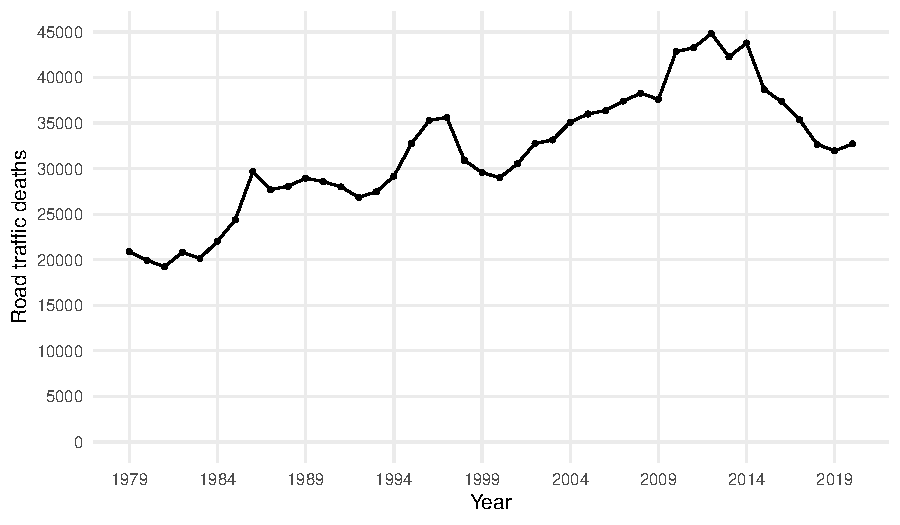
\includegraphics{fig/brazil_abs.pdf}
    \label{fig:br_abs}
    \par SOURCE: The Author, based on \textcite{MinistryofHealth2020}.
\end{figure}

The year of 1979 is the earliest official data entry available. Starting in the 1980s, there is a overall rising trend in the numbers of road traffic deaths that reach its peak in 2012, then it starts declining. In 2010, the year before the Decade of Action, Brazil had 42,844 deaths and reached the max value in 2012: 44,812 road traffic deaths. Almost at the end of the decade the number of deaths declined, reaching 31,945. The next plot (\autoref{fig:br_mort}) shows the mortality rate in Brazil, considering the same time span. In general, it follows the same pattern of the absolute road traffic deaths.

\begin{figure}[!htbp]
    \centering\footnotesize
    \captionsetup{font=footnotesize}
    \caption{ROAD TRAFFIC MORTALITY RATE ON BRAZIL}
    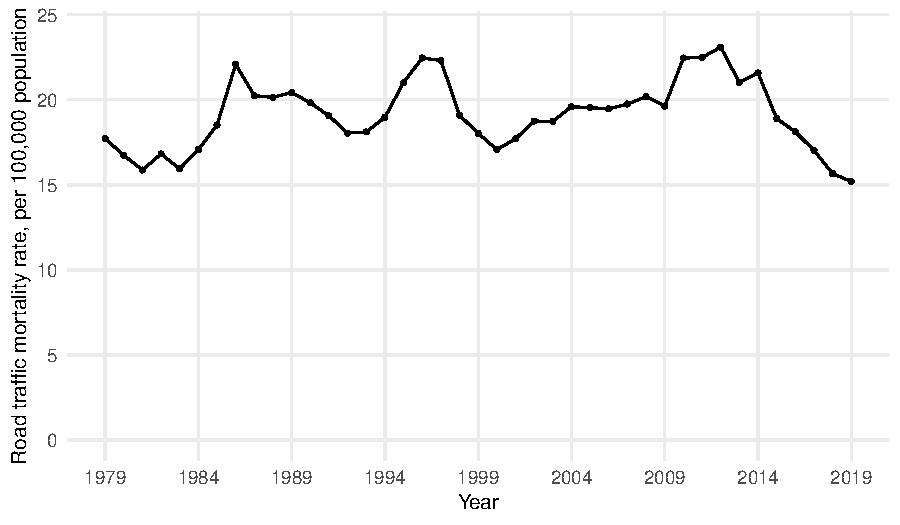
\includegraphics{fig/brazil_mort.pdf}
    \label{fig:br_mort}
    \par SOURCE: The Author (2021), based on \textcite{MinistryofHealth2020} and \textcite{MinistryofHealth2021}.
\end{figure}

The maximum registered mortality rate is 23.1 deaths per 100,000 inhabitants in 2012, the same year which Brazil reached its maximum value for absolute road traffic deaths. Since then the mortality rate has been declining, reaching a rate of 15.2 deaths per 100.000 inhabitants in 2019. In comparison to the OECD countries (\autoref{fig:oecd}), Brazil presented a strong declining pattern a few years later, after the 2010s. Another indicator that considers the exposition to traffic hazards is the fatality rate - number of deaths per 10,000 vehicles (\autoref{fig:br_fatal}). The oldest entry of fleet size in the \textcite{DENATRAN2020} database is 1998.

\begin{figure}[!htbp]
    \centering\footnotesize
    \captionsetup{font=footnotesize}
    \caption{ROAD TRAFFIC FATALITY RATE ON BRAZIL}
    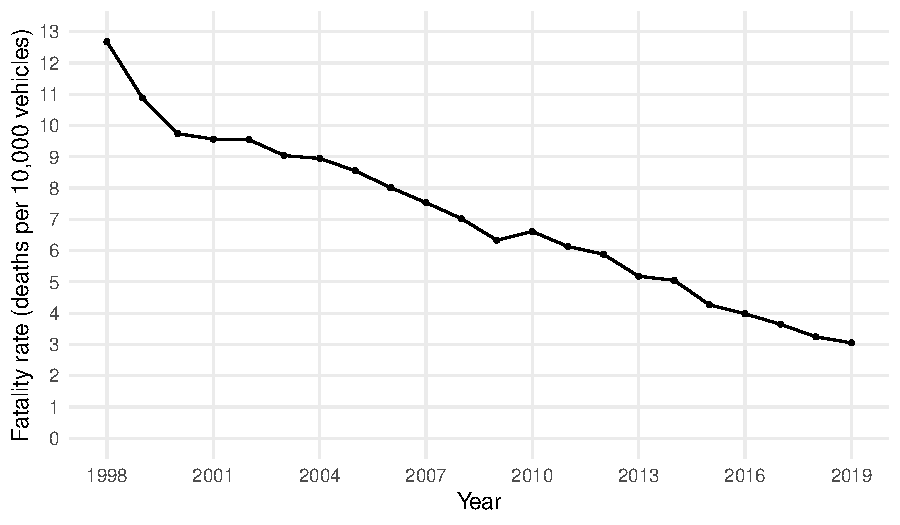
\includegraphics{fig/brazil_fatality.pdf}
    \label{fig:br_fatal}
    \par SOURCE: The Author (2021), based on \textcite{MinistryofHealth2020} and \textcite{DENATRAN2020}.
\end{figure}                                

Between 1998 and 2019 there is a declining pattern in the fatality rate, starting with 12.7 deaths per 10,000 vehicles in 1998 and ending with 3.0 in 2019, representing a reduction of 76\%. This declining pattern can be explained by the continuous rise of the motorization rate (\autoref{fig:br_motor}). In 1998, the motorization rate was 151 vehicles per 1,000 population, increasing to the rate of 499 in 2019. The motorization can be defined as one indicator of the development un the country. Considering the motorization stages defined by \textcite{Jorgensen2005}, Brazil can be classified nowadays with a exploding motorization. 

The first stage of motorization - developing motorization - occurs when a country have a motorization rate between 50 and 100 vehicles per 1,000 inhabitants. This first stage happened in Brazil before 1998. The explosion of the motorization is the second stage, and it happens with a motorization rate of between 300 and 400. The third and last stage is the saturation, and occurs when the motorization rates reaches more than 400 and its tendency stops rising \cite{Jorgensen2005}. Although Brazil has a present motorization rate above 400, it is plausible to affirm that the country still hasn't reached the stage of saturation, considering that the rates are still in a rising pattern. 

\begin{figure}[!htbp]
    \centering\footnotesize
    \captionsetup{font=footnotesize}
    \caption{MOTORIZATION RATE ON BRAZIL}
    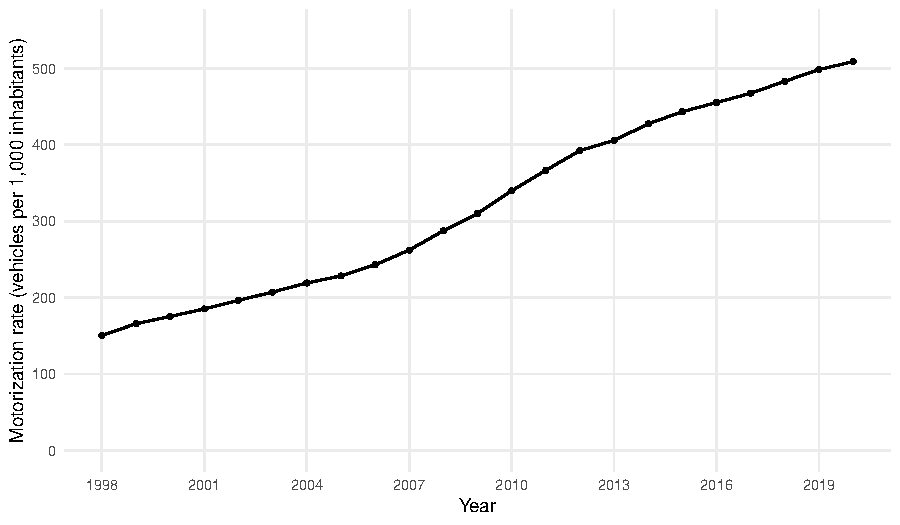
\includegraphics{fig/brazil_motor.pdf}
    \label{fig:br_motor}
    \par SOURCE: The Author (2021), based on \textcite{MinistryofHealth2021} and \textcite{DENATRAN2020}.
\end{figure} 

In the 1970s, Brazil have undergone through a intense development in the car industry, lowering the price of the vehicles and increasing the development of road infrastructure in cities and rural areas, impacting directly in the rise of the motorization in the country \cite{Vasconcellos2013}. To \textcite{Harvey1982}, this incentive to motorization created a urban environment that looked to answer the increasing demand of car use. This process lead to worse safety conditions in brazilian cities, specially to non motorized users in the road system.   

The variation in the number of road traffic deaths and road traffic mortality heavily influenced by the socioeconomic development and political landscape \cite{Ferraz2012}. The country had different economical situations between the 2000s and the 2010s. In the period of 2000-2010, Brazil had a continuous growth in the economy, which reflected on the rising pattern of the road traffic deaths and road traffic mortality rates. After the 2010, the country entered in a economic recession, leading to the reduction of these numbers \cite{Bastos2020}. Focusing on the area of study, the road traffic deaths in Curitiba are presented in \autoref{fig:cwb_abs}.   

\begin{figure}[!htbp]
    \centering\footnotesize
    \captionsetup{font=footnotesize}
    \caption{ROAD TRAFFIC DEATHS ON CURITIBA}
    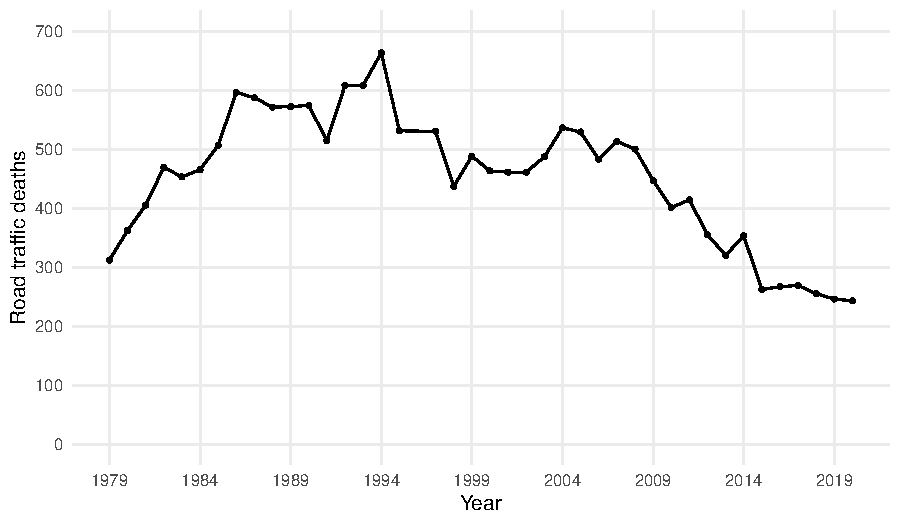
\includegraphics{fig/cwb_abs.pdf}
    \label{fig:cwb_abs}
    \par SOURCE: The Author (2021), based on \textcite{MinistryofHealth2020}.
\end{figure}  

The tendency of road traffic deaths presented a rising pattern between 1979 and 1994, starting with 312 deaths and reaching a maximum of 663 deaths. Overall, the pattern of the time series started declining after 1995, ending with a minimum value of 246 in 2019. Following the brazilian trend, Curitiba's motorization rate kept rising in the last decades. The increase in motorized transit can lead to more exposition to traffic crashes and injuries, in case road safety interventions are not implanted correctly. The plot in \autoref{fig:cap_motor} compares the motorization rate between all brazilian states capital cities.    

\begin{figure}[!htbp]
    \centering\footnotesize
    \captionsetup{font=footnotesize}
    \caption{MOTORIZATION RATES ON BRAZILIAN STATES CAPITAL CITIES, IN 2019}
    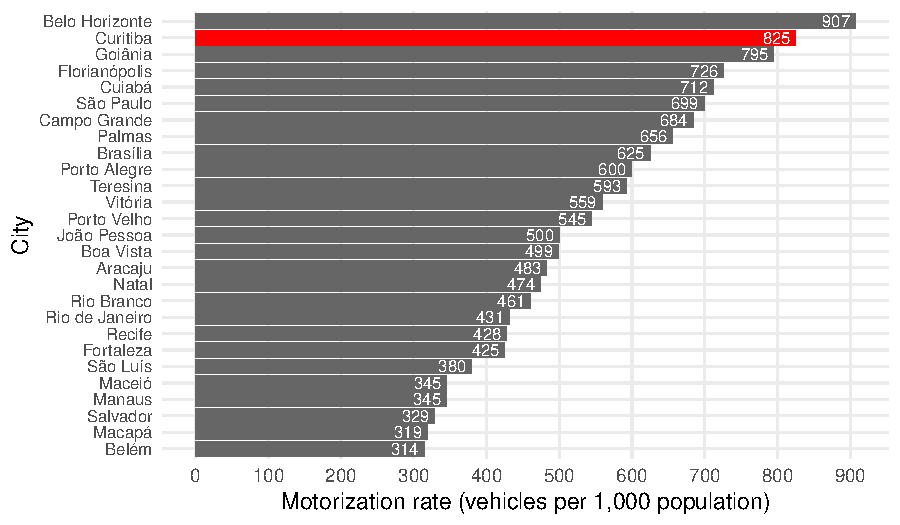
\includegraphics{fig/cap_motor.pdf}
    \label{fig:cap_motor}
    \par SOURCE: The Author (2021), based on \textcite{MinistryofHealth2021} and \textcite{DENATRAN2020}.
\end{figure}   

Curitiba was, in 2019, the second most motorized capital in Brazil, with a motorization rate of 825 vehicles per 1,000 population, higher than the brazilian average, losing only to Belo Horizonte, which presented a motorization rate of 907 vehicles per 1,000 population. When comparing the road traffic mortality rate (\autoref{fig:cap_mort}), Curitiba stays in the 13th place with 12.7 deaths per 100,000 inhabitants, below the brazilian average of 15.2 in 2019. The lowest value of road traffic mortality rate belongs to Rio de Janeiro, presenting a rate of 5.7 deaths per 100,000 population, and the highest belongs to Palmas, with a alarming rate of 36.4. In 2015, Curitiba had a mortality rate of 13.94 deaths per 100,000 inhabitants, a higher value when comparing to more developed countries, like Sweden (2.8), UK (3.1) and Germany (4.1). Curitiba's rate for 2015 has a similar value to other latin american countries: Mexico (13.1), Uruguay (13.4), Peru (13.5) and Argentina (14.00) \cite{WHO2018}. 

\begin{figure}[!htbp]
    \centering\footnotesize
    \captionsetup{font=footnotesize}
    \caption{MORTALITY RATES ON BRAZILIAN STATES CAPITAL CITIES, IN 2019}
    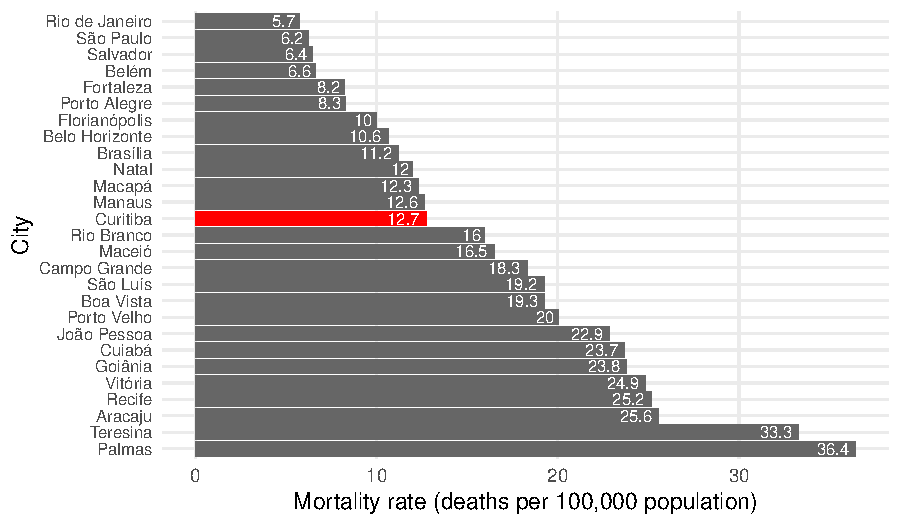
\includegraphics{fig/cap_mort.pdf}
    \label{fig:cap_mort}
    \par SOURCE: The Author (2021), based on \textcite{MinistryofHealth2020} and \textcite{MinistryofHealth2021}.
\end{figure}  

Considering the fatality rate as a road safety performance indicator, \autoref{fig:cap_fatal} plot shows that Curitiba have the 6th best performance, with a fatality rate of 1.5 deaths per 10,000 vehicles. São Paulo is the capital with the lowest fatality rate (0.9) and Recife has the highest one (5.9). Observing the fatality rate in Brazil in the same period (3.0), Curitiba is below the country average, with exactly 50\% less deaths per 10,000 vehicles. Road traffic crashes and its related injuries have become a serious health problem across brazilian cities. As motorization increases, the number of conflicts and possible crashes increases as well.

\begin{figure}[!htbp]
    \centering\footnotesize
    \captionsetup{font=footnotesize}
    \caption{FATALITY RATES ON BRAZILIAN STATES CAPITAL CITIES, IN 2019}
    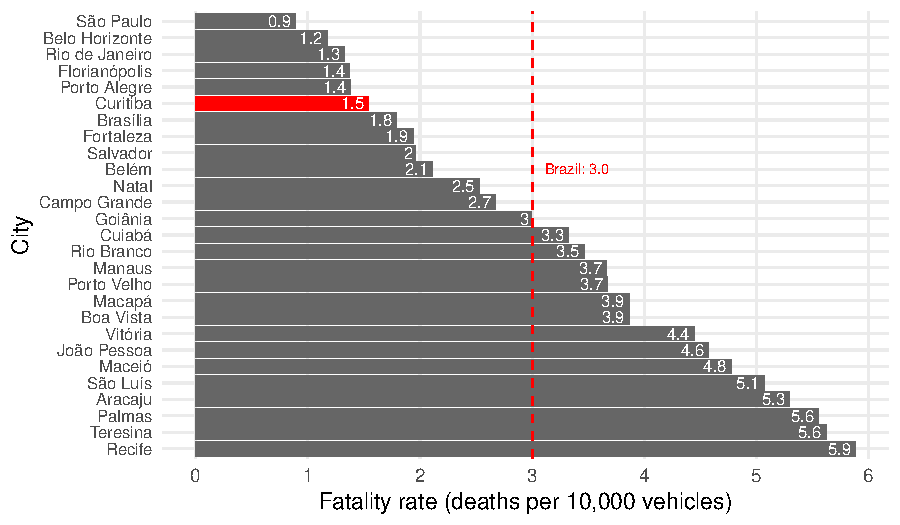
\includegraphics{fig/cap_fatal.pdf}
    \label{fig:cap_fatal}
    \par SOURCE: The Author (2021), based on \textcite{MinistryofHealth2020} and \textcite{DENATRAN2020}.
\end{figure} 

Capable interventions in road safety needs to consider traffic deaths and injuries as serious public health problems. Therefore, its control must follow the principle as control of any other public health problem. Road traffic injuries are the result of a complex interaction of multiple factors. These factors can involve human, environmental and vehicle factors, in addition to sociological, psychological, physical and technological factors present the process of traffic crashes. As another health problems, it is possible to analyze road traffic injuries considering three different phases in time: pre-crash, during the crash and post-crash \cite{Mohan2016}.

These distinct phases of time and factors of road traffic crashes can be arranged into a matrix created by \textcite{Haddon1980} in order to map all events related to a injury. Named after its inventor, the Haddon matrix (\autoref{fig:haddon}) consists of two dimensions: one for the time aspect of the event and a second one representing three main discrete factors: human, vehicle and environment. Crossing each step of both dimensions sets nine cells, in which can be made a list of countermeasures to control the damage or to prevent a possible incident, associating these measures to each pair of factors. 

\begin{figure}[!htbp]
    \centering\footnotesize
    \captionsetup{font=footnotesize}
    \caption{HADDON MATRIX}
    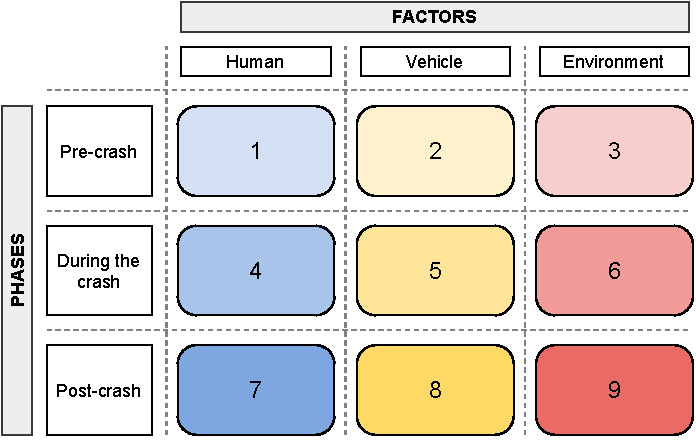
\includegraphics{fig/haddon.pdf}
    \label{fig:haddon}
    \par SOURCE: The Author (2021), based on \textcite{Haddon1980}.
\end{figure} 

Cells 1, 2 and 3 contains measures towards the prevention of crashes. On a road traffic crash scenario, cell 1 considers the behavior (aggressive driving, driving under influence, distraction) and training of the road users (pedestrians, drivers, motorcyclists and cyclists), cell 2 presents safety interventions related to the vehicles (use of daylight headlights, speed control systems, etc.) and cell 3 contains all elements of the road infrastructure the and build environment that influences directly into the occurrence of this event. Cells 4, 5 and 6 comprehends measures that can reduce the severity during the occurrence of a crash event.

In cell 4 there are measures that include the use of seat belts, helmets and protective clothing. Cell 5 can consider the crashworthiness and safety design of the vehicles and cell 6 includes elements (or lack of elements) that can influence the severity in case of a collision (guard rails, concrete barriers, street furniture, etc.). In the last row are included the measures related to the control and treatment of injuries after the event. Cell 7 presents the treatments related to the victims (hospital care and rehabilitation), cell 8 contain measures related to the safety systems of a vehicle and cell 9 can consider the general management of a crash scene \cite{Mohan2016}. 

The road safety problems that happens on urban environments may differ from the ones that happens in major roadways. Even with lower operating speeds, the quantity of conflicts in urban road systems can be considerable higher when comparing to rural roadways, considering the quantity of different motorized and non-motorized transport modes that uses the infrastructure in the same time. Consequently, it is essential to follow requirements for a safe infrastructure. Three main ones are functionality, homogeneity and recognition \cite{SWOV2003}. Each road on a network needs to have a specific function (balance between mobility and access), with traffic distribution working as intended. Homogeneity consists in reducing the points of conflict between transport modes with great difference of mass and speed. Finally, the situations on traffic should have a level of predictability, passing what behavior should be expected from the road users.

In order to reduce road traffic crashes and possible consequent injuries or deaths, it is relevant to consider the main risk factors that causes and intensify these events. According to \textcite{WHO2004}, risk in road traffic can be classified into four elements which are directly influenced: exposure, crash involvement, crash severity and post-crash severity. The risk factors that can be classified in these elements also can be distributed within the Haddon matrix as well \autoref{fig:haddon}. The main risk factors related to the protection of the user consists in the usage of seat belts, helmets, air bags, child restraints and helmets. Focusing on the behavioral factors, the main ones are driving under influence of alcohol and another drugs (DUI), distraction and inattention \cite{Shinar2017}.

The excess of speed and the speed differential in urban environments are two risk factors that affects the chance of traffic crashes occurrence and the severity of theses crashes. Speeding is a complex phenomenon with multiple causes, consequences and methods of prevention. Given its complexity and spotlight in this thesis, this risk factor will be discussed in the next section (\ref{speeding}). 

\section{SPEEDING AS A RISK FACTOR} \label{speeding}

Speeding is one of the primary global causes of road traffic fatalities, affecting two main dimensions: probability and severity \cite{WHO2013}. The increase in speeds of vehicles is directly correlated to the increase in the occurrence of crashes and its average severity, hence, strongly related to the road safety \cite{Mohan2016a}. Another speed-related risk factor is the speed differential, which is the speed deviation from the average operating speed \cite{Shinar2017}. \textcite{Ferraz2012} defines speeding as a inappropriate speed, leading to more conflict and crashes in certain traffic conditions. 

The excess of speed can influence three main factors in the occurrence of a traffic conflict: reaction time, braking distance and force of impact, which is directly correlated to the severity of injuries \cite{Mohan2016a}. Reducing the speed helps the driver to increase its reaction time, also helping the driver to take a correctional action to anticipate crashes \cite{Elvik2009}. Regarding the braking distance, lower speeds reduces the distance necessary to fully stop the vehicle. \autoref{fig:braking} shows the reaction time of a vehicle added to the braking distance, resulting in the distance travelled by the vehicle. The dashed line represents a pedestrian standing 35 meters from the traveling vehicle. 

\begin{figure}[!htbp]
    \centering\footnotesize
    \captionsetup{font=footnotesize}
    \caption{RELATIONSHIP BETWEEN SPEED AND BRAKING DISTANCE}
    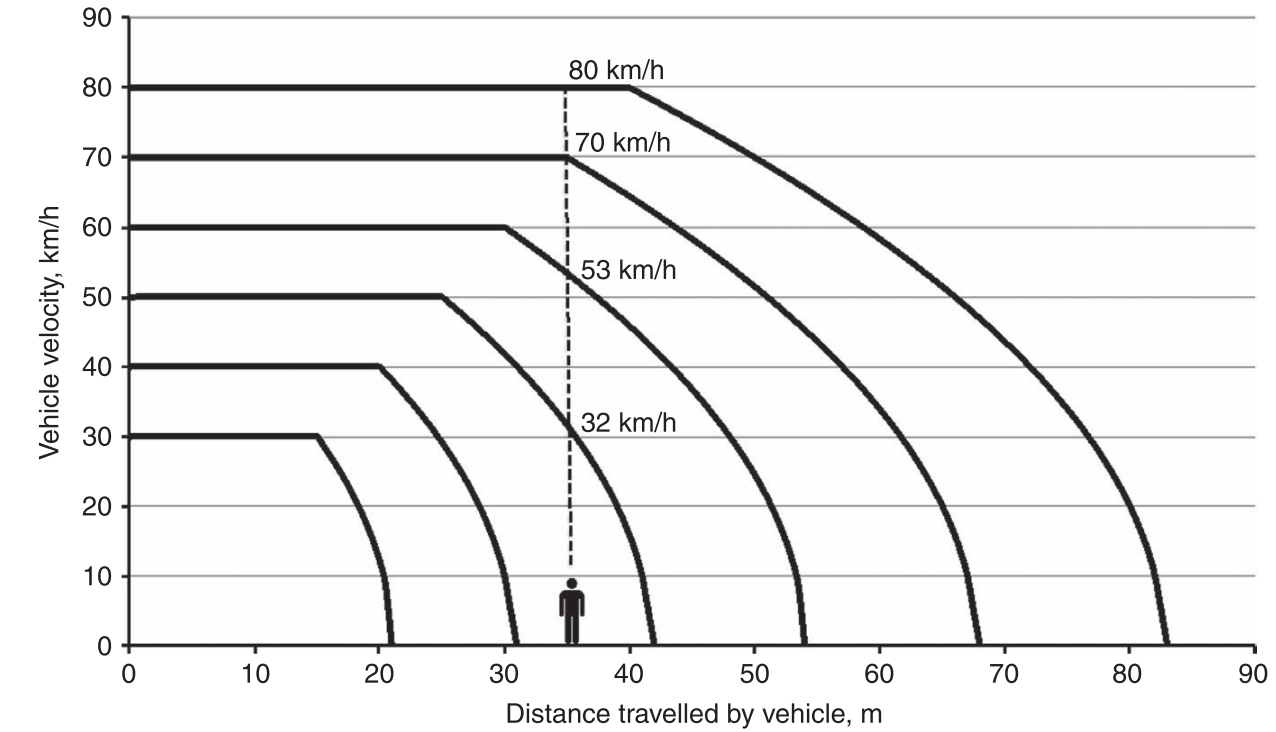
\includegraphics[width=0.8\textwidth]{fig/braking2.png}
    \label{fig:braking}
    \par SOURCE: \textcite{Mohan2016a}.
\end{figure} 

The horizontal lines from the plot shows the cruising speeds of the vehicle before they start breaking, longer lines at higher speeds represents greater reaction times. In this scenario, only speeds equal or below 40 km/h are able to avoid a collision with the pedestrian. As the vehicle speed rises, the impact speed rises as well. This leads to the increase in force of impact between vehicles and pedestrians. The severity of injuries sustained by pedestrians depends on the energy of impact - the kinetic energy transferred to the human body. This energy of an object (the vehicle), directly related to its velocity and mass, detailed in the following equation: \begin{align}
    E = 0.5 \times MV^2 \mbox{;}
    \label{eq:energy}
\end{align} where $E$ is the kinetic energy, $M$ is the object's mass and $V$ is the velocity of the object. The plot in \autoref{fig:kinetic} shows the increase in kinetic energy, considering an average car mass of 1,500 kg \cite{Zervas2008} and speeds varying between 0 and 100 km/h. The quantity of energy doubles when the speed changes from 40 km/h to 60 km/h, and almost triples at 70 km/h. This variation shows how the reduction of speed limits can greatly change the energy of impact.

\begin{figure}[!htbp]
    \centering\footnotesize
    \captionsetup{font=footnotesize}
    \caption{RELATIONSHIP BETWEEN SPEED AND KINETIC ENERGY}
    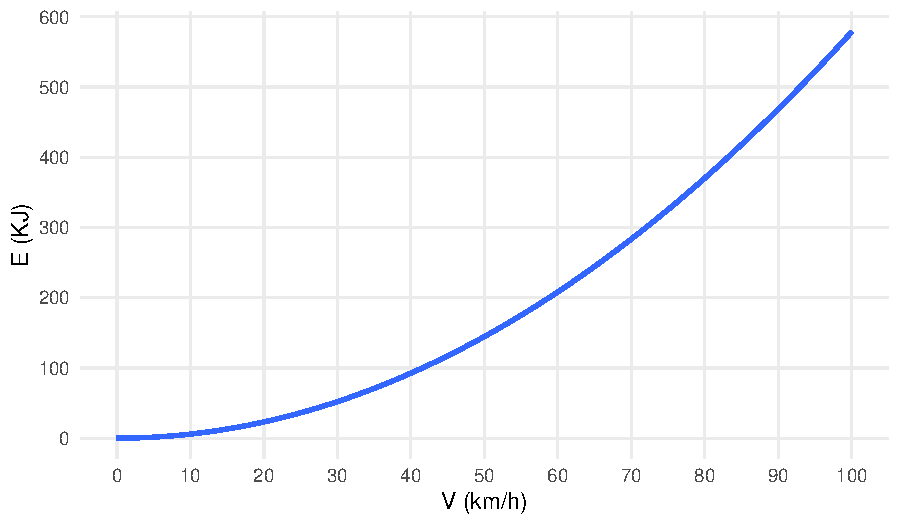
\includegraphics{fig/kinetic.pdf}
    \label{fig:kinetic}
    \par SOURCE: The Author (2021).
\end{figure}

Considering the event of an impact between a front of a car and a pedestrian, \textcite{Ashton1980} presented the relationship between the impact speed and the percentage of fatally injured pedestrians per speed window, represented in the plot of \autoref{fig:ash}. The curve shows how a reduction from 60 km/h to 40 km/h on the speed of impact can reduce the chance of a fatal injury from 90\% to 30\%, approximately. Reducing the speed of impact to 30 km/h will reduce the chance of a fatal injury to approximately 10\%. In general, as the speed of impact rises, the chance of a fatal injury rises too, with a greater variation between speeds of 30 km/h and 60 km/h. 

\begin{figure}[!htbp]
    \centering\footnotesize
    \captionsetup{font=footnotesize}
    \caption{PROBABILITY OF PEDESTRIAN FATALITY AT DIFFERENT IMPACT FATALITIES}
    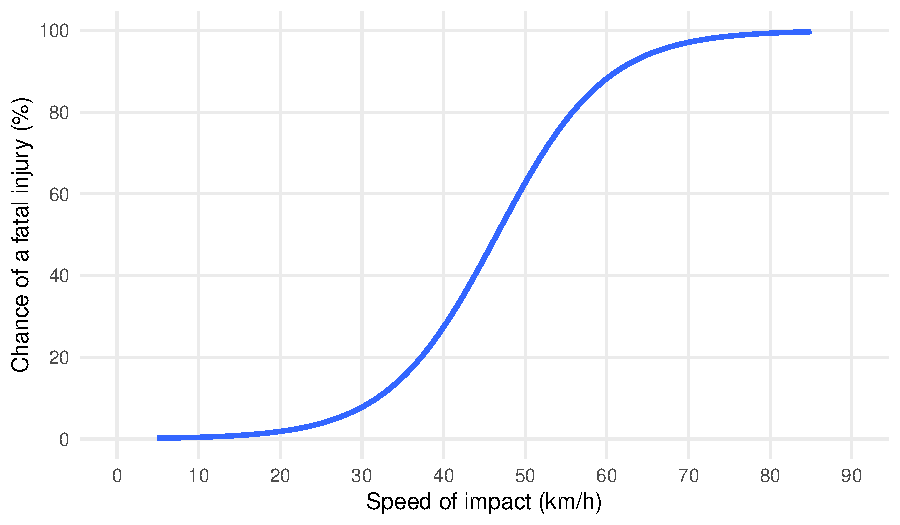
\includegraphics{fig/ash.pdf}
    \label{fig:ash}
    \par SOURCE: The Author (2021), based on data from \textcite{Ashton1980}.
\end{figure}

The risks highlights the importance of proper speed management in road traffic, specially in urban environments. Roadways have higher operational speeds, but cities contains a more expressive interaction between motorized and vulnerable users, in which lower speeds can still represent a risk to pedestrians and cyclists. One method to manage the operating speed is the enforcement of speed limits. It is recommended a speed limit of 50 km/h in urban arterial roads, and a limit of 30 km/h in roads with a high flow of pedestrians and cyclists \cite{WHO2008}. Reducing the mean speeds can greatly favor the decline in fatal, non fatal and property damage only (PDO) road crashes \cite{Elvik2013}. 

The operating and mean speed of the road traffic depends on how the drivers chooses the speed. This choice is related to the power and stability of the user's vehicle, to road and traffic conditions,to  driver's perception of safety, to the level of enforcement, travel motivations, personal characteristics and behavior of other drivers \cite{Mohan2016a, Shinar2017}. Considering all theses factors, it is not effective to rely only on traffic limits to prevent speeding. If the design speed of a road is higher than the speed limit and the road traffic has a low density, it is more difficult to enforce a the desired limit. The difficulty to enforce the speed limits may be higher to LMICs, which have less resources to adopt the proper road designs policies and enforcement levels required to this task \cite{Mohan2016a}. 

In \autoref{tab:spdfct} is presented a few groups of factors affecting speeding and speed choice, with its categorization based on the three main discrete factors of road crashes established by \textcite{Haddon1980}: human, vehicle and environment. Analyzing the human (or driver) factors, the background characteristics includes the level of experience, education and training of the drivers. Demographic characteristics considers the groups of age, sex and income. The general health of the driver, including the conditions of vision, hearing and sleep patterns are included in the physiological factors. The last factor in the human group - attitudes, beliefs and motivations considers how the road user perceives the control and norms present in traffic situations \cite{Richard2013a}.  

\begin{table}[!hbtp]
    \footnotesize
    \captionsetup{justification=raggedright,
        singlelinecheck=false,
        font=footnotesize}
    \caption{FACTORS THAT AFFECTS SPEEDING AND SPEED CHOICE}
    \centering
    \begin{tabular}{lll}
    \hline
    \multicolumn{1}{c}{\textbf{Human}}                  & \multicolumn{1}{c}{\textbf{Vehicle}} & \multicolumn{1}{c}{\textbf{Environment}} \\ \hline
    Background characteristics      & Type/Size        & Road elements        \\
    Demographic characteristics     & Engine power     & Weather              \\
    Physiological factors           & Comfort          & Traffic conditions   \\
    Attitudes, beliefs and motivations & Field of view    & Surroundings    \\
                                    & Age              & Speed Enforcement    \\ \hline
\end{tabular}
    \label{tab:spdfct}
    \par \vspace{2mm} \footnotesize \raggedright
    SOURCE: The Author (2021), based on \textcite{Richard2013a}, \textcite{Shinar2017} and \textcite{WHO2008}.
\end{table}

All these human factors are related to the general driver profile and its performance when driving the car. as an example of the influence in the individual differences present in the demographic characteristics, younger drivers are more likely to speed than mature and older drivers, and men are more likely to speed than women \cite{Shinar2017}. The vehicle characteristics also affects the speed choice of the user. The type, engine power, comfort, field of view and age of the vehicle can affect the possibility to the driver reach the desired speed. 

The environmental factors affecting speed choice consists of all the elements external to the vehicles and are greatly related to how the driver behaves and to how the vehicle is able to operate. Road elements can include the general characteristics of a road layout, quantity and type of intersections, design and level of maintenance, based on its alignment, gradient, width, surface condition, geometric pattern and road lightning. The presence of intersections and the high density of traffic controls the operating speeds in urban areas \cite{Mohan2016a}. Weather can also affect how the driver will chose his speed, considering its effects on surface conditions (dry, wet, ice) and natural light.  

The speed and speed variance are to a certain extent determined by the traffic flow regime \cite{Shinar2017}. Depending on the level of flow and density or any other operational condition of the traffic, the driver cannot be able to reach a higher desired speed, removing his ability to have a opportunity to speed \cite{Richard2013a, Bastos2021}. The plot in \autoref{fig:svd} illustrates the relationship between speed, density and volume (or flow) in uninterrupted flow conditions of a certain road. This type of flow occurs in areas without interference from external factors, like intersections or crossings \cite{Green2020}. 

\begin{figure}[!htbp]
    \centering\footnotesize
    \captionsetup{font=footnotesize}
    \caption{RELATIONSHIP BETWEEN TRAFFIC SPEED, VOLUME AND DENSITY}
    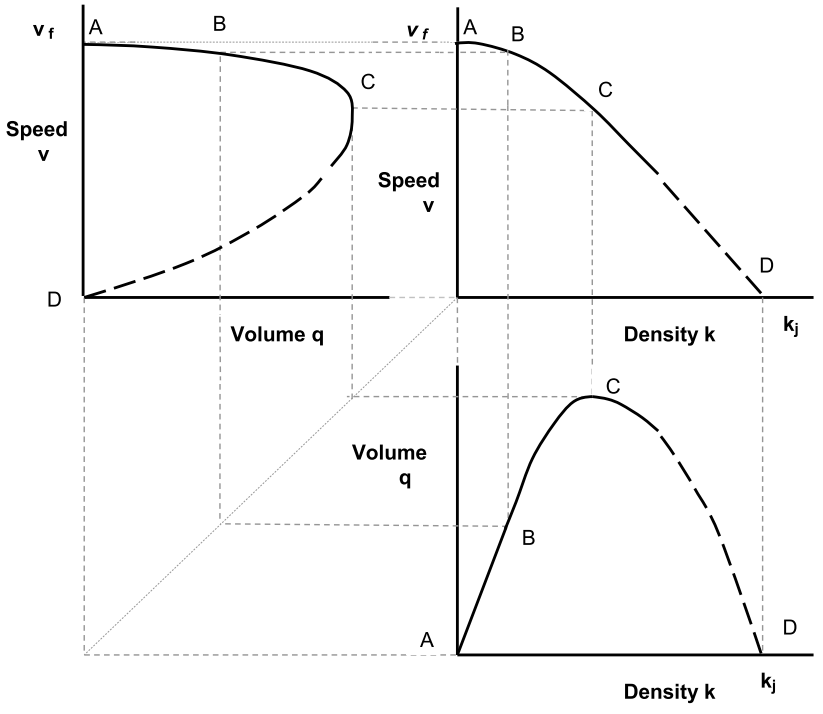
\includegraphics[width=0.8\textwidth]{fig/svd.png}
    \label{fig:svd}
    \par SOURCE: \textcite{Green2020}.
\end{figure}

When density and volume are at its lowest value, the road user can reach higher speeds without having traffic to prevent it (point A). Between points A and B, volume and density starts to rise and speeds decline a little, but still is high enough to be characterized as a free flow speed. In this situation, the driver starts to experience a lack of manoeuvre freedom, but it still have the opportunity to speed. At the highest level of density (point C), speed declines as density rises. Between C and D, density rises until it reaches its maximum value, reducing overall speeds and volume \cite{Green2020}. In this last stage, the drivers have less flexibility to choose a desired speed, having to operate in a forced flow condition. 

Established as an environmental factor affecting speeding choice (\autoref{tab:spdfct}), the surroundings of the road, including equipments and some traffic calming techniques like gateway treatments, can be perceived by the driver as elements that gives hints to avoid higher speeds \cite{WHO2008}. Overall, the built environment and its five elements - density, design, diversity, destination accessibility and distance to transit - can be perceived as environmental factors which affects the road safety, through the relationship to the numbers of road crashes and occurrence of speeding. These characteristics are better explored in the next section (\ref{be}). 

In order to collect speeding data, it is important to establish what defines speeding and to identify a measure of exposure to speeding. To \textcite{Richard2013}, defining speeding and its constitution is one of the key challenges of speeding studies. The authors presented five distinct approaches for defining speeding: ad hoc, analytical, kinematic, psychological and behavioral. The ad hoc approach assumes that the fastest driving in a sample if a proxy for speeding and considers the top X\% of speeds above the posted speed. Although this approach can provide sufficient data for analysis, the speeding collected may be not related to behavior or safety. 

The analytical approach fixes a criterion relative to the speed limit (+ X\% or + X km/h). It is a simple method to implement, but can miss some factor related to road type and overall speed level. The analytical approach is used in this work and its process of implementation is detailed in Section \ref{data}. The kinematic approach considers the driving environment and its operational conditions, in order to connect the speed behavior to specific situations. This approach requires a certain level of quantity and quality of GIS data to support it. The psychological approach is based on what the driver considers to be speeding, providing insight into factors that are related to individuals perception of speeding. The necessity of additional previous information about the speeding beliefs and attitudes of the drivers can be a disadvantage of this approach. At last, the behavioral approach sets four speed bands to describe different behavior in each one, related to the chosen speed by the driver \cite{Richard2013}.

The operational aspects of urban road traffic (mostly in interrupted flow conditions) arbitrary reduces the amount of speeding being measured. To address this problem, it is necessary to extract the free-flow situations of the trip from the total trip distance, removing sections in which drivers had no opportunity to speed. This process of extracting parts of the trip in which the driver is exposed to speeding is presented in \autoref{fig:ff}. Therefore, the actual measure of speeding is distance performed in speeds above the posted speed compared to the distance performed in free-flow speed. This process was applied in this work and it is described in Section \ref{data}. 

\begin{figure}[!htbp]
    \centering\footnotesize
    \captionsetup{font=footnotesize}
    \caption{EXTRACTION OF FREE-FLOW AND SPEEDING EPISODES FROM TRIPS}
    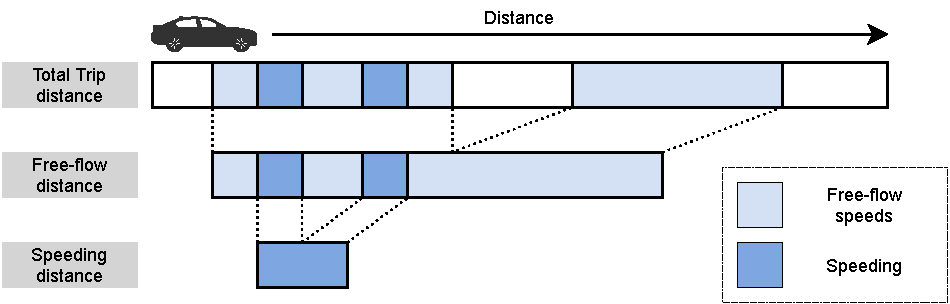
\includegraphics{fig/richards.pdf}
    \label{fig:ff}
    \par SOURCE: The Author (2021), based on \textcite{Richard2013}.
\end{figure}

The data collected also depends on the method applied. The collection of speed data can be done with the use of speed traps - fixed or mobile \cite{Hidalgo-Solorzano2020, WHO2008}, the analysis of road crashes reports \cite{Watson2015}, roadside observational studies \cite{Shinar2017}, questionnaires \cite{Dinh2013}, smartphone data \cite{Warren2019} and GPS data collection \cite{Moreno2013, Wang2018}. Studies that uses naturalistic data includes the capture video data from the drivers and GPS can relate the speeding action registered with a certain behavioral action from drivers \cite{Bastos2020a} and environmental factors \cite{Moreno2013}. The speeding data collected from driving simulation studies also can be correlated with other environmental or behavioral factors \cite{Yadav2020}. The aspects of naturalistic driving studies and its comparison to other methods will be better explored in the Section \ref{nds}. 

Knowing the factors that affects speeding and the methods to collect and analyse speeding data, it is possible to create countermeasures to this risk factor in road traffic crashes. Following the categories established by \textcite{Haddon1980} and presented in \autoref{tab:spdfct}, these countermeasures can be classified into behavioral (human), vehicular and environmental approaches. Behavioral approaches includes the education and training to teach speed awareness to drivers. Enforcement is also a behavioral approach. Enforcement by the police or other traffic authority is related to a greater rate of speed limit compliance, but it is a highly localized measure \cite{Shinar2017}. 

The vehicle approach to intervene in speeding practices includes speed limits and advisory systems in cars. Environmental approaches are consisted of direct changes in infrastructure, including traffic calming measures, and policy approaches, including the establishment of speed limits and administrative actions. Speed bumps, lane narrowing, roundabouts and rumble strips are some of the traffic calming techniques that are capable to reduce speeds in urban environments \cite{Welle2016}. Other key elements of urban design also can intervene in the practice of speeding, including street block sizes, road network connectivity and road lane width.

\section{ROAD SAFETY PERFORMANCE AND THE BUILT ENVIRONMENT} \label{be}

% 1. Introduce the section with Tiwari (2016) and Ewing (2009)

%% Ewing and dumbaugh diagram

%% Tiwari 

%% Ewing and Cervero, 2010

The built environment consists of the physical elements and features, including the development patterns and the roadway designs of a city. Built environment affects the physical activity inside the city, including the overall mobility, road safety and health. According to \textcite{Ewing2009}, the frequency and severity of road traffic crashes are related to the built environment through three mediators: traffic volumes, traffic conflicts and traffic speeds, as shown in \autoref{fig:ewing}. Therefore, the land use and transport plans influences the choice of destination, travel models, travel distances and routes, impacting the road traffic safety \cite{Tiwari}.  

\begin{figure}[!htbp]
    \centering\footnotesize
    \captionsetup{font=footnotesize}
    \caption{BUILT ENVIRONMENT AND TRAFFIC SAFETY}
    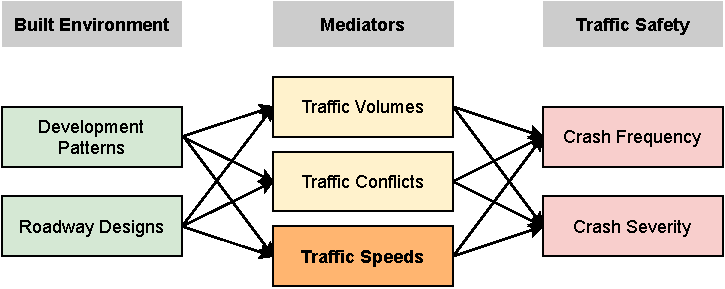
\includegraphics{fig/ewing.pdf}
    \label{fig:ewing}
    \par SOURCE: The Author (2021), based on \textcite{Ewing2009}.
\end{figure}

Traffic volume is directly related to crash frequency and the increase of vehicle miles travelled (VMT), which is a exposure variable to the occurrence of road traffic crashes. Traffic speed (and its excess), the main factor investigated in this paper, is affected by the operating and encouraged speed defined by the roadway design and development pattern. Traffic conflicts are related to the increase in vehicle flow and traffic speed \cite{Ewing2009}. Overall, the built environment can be characterized into five ``D'' variables: (\romannumeral 1) density, (\romannumeral 2) diversity, (\romannumeral 3) design, (\romannumeral 4) destination accessibility and (\romannumeral 5) distance to transit, being defined as the 5D \cite{Ewing2010}. Demographics of residents, while not being part of the built environment, can be considered as the sixth ``D''. 

% 2. Describe the BE elements. (5D)

%% Table with 5D and elements used in this work

%% Other reports from Tiago

%% Tiwari

\autoref{tab:6d} contains the categories previously described and its variables. It is important to note that it is not presented all the possible built environment variables, only the main ones found in previous papers. In addition, these are rough categories, divided by boundaries that are subject to change \cite{Ewing2010}. Density measures a variable of interest per unit of area and can include the quantity of population, housing or number of jobs, showing the ``hotspots'' of the overall activity in a city. Diversity refers to different land use types within a given area, ranging from single-use environments to more varied land uses. The street network and its characteristics is included in the design category, and considers elements like block size, type / quantity of intersections, street widths, quantity of pedestrian crossings and street network density.

\begin{table}[!hbtp]
    \footnotesize
    \captionsetup{justification=raggedright,
        singlelinecheck=false,
        font=footnotesize}
    \caption{BUILT ENVIRONMENT VARIABLES}
    \centering
    \begin{tabular}{ll}
        \hline
        \multicolumn{1}{c}{\textbf{Category}}                          & \multicolumn{1}{c}{\textbf{Variable}}                        \\ \hline
        \multirow{3}{*}{Density}                   & Population                               \\
                                                   & Housing                                  \\
                                                   & Employment                               \\ \hline
        \multirow{1}{*}{Diversity}                 & Land use                                 \\
                                                   \hline
        \multirow{6}{*}{Design}                    & Block size                               \\
                                                   & Type / Quantity of intersections                \\
                                                   & Street widths                            \\
                                                   & Quantity of pedestrian crossings         \\
                                                   & Road hierarchy \\
                                                   & Street network density \\
                                                    \hline
        \multirow{3}{*}{Destination Accessibility} & Quantity of commercial and service units \\
                                                   & Distance to city center                  \\
                                                   & Quantity of jobs                         \\ \hline
        \multirow{2}{*}{Distance to Transit}       & Quantity of bus stops                    \\
                                                   & Distance to nearest transit stop         \\
                                                    \hline
        \multirow{3}{*}{Demographics}              & Income                                   \\
                                                   & Age                                      \\
                                                   & Sex                                      \\ \hline
        \end{tabular}
    \label{tab:6d}
    \par \vspace{2mm} \footnotesize \raggedright
    SOURCE: The Author (2021), based on \textcite{Ewing2009}, \textcite{Ewing2010} and \textcite{Obelheiro2020}.
\end{table}

Destination accessibility measures how easy is to access places of attraction, including jobs, services, commerce and districts of overall interest, considering business districts and city downtown. Distance to transit usually is measured by the level of offer of transport services, being measured by the quantity of transit stops and network density. Network density also can be included in the design category. Demographics, while not being a characteristic of the build environment, can influence the occurrence of speeding in urban environments, including income, age and sex. In the following tables (\autoref{tab:density} to \autoref{tab:demographics}) are presented the built environment categories and its variables considered in this work, considering the authors that investigated them related to the road safety performance in urban areas, with the focus on one final outcome indicator - road crashes and one mediator - occurrence of speeding.

% 3. BE and relationship to road safety

%% table with all the authors

\autoref{tab:density} displays a list of authors which investigated the relationship between population density and road safety in urban areas. Regarding road traffic crashes, \textcite{Dumbaugh2009, Obelheiro2020} found a inverted correlation between number of habitants per area and occurrence of road crashes. Higher densities environments causes people to drive less \cite{Dumbaugh2009}, reducing the exposure to road traffic accidents. A research considering road safety and BEs about another brazilian city - Porto Alegre - also presented a result of a inverted relationship between injury crashes and population density in most of the city's area.

\begin{table}[!hbtp]
    \footnotesize
    \captionsetup{justification=raggedright,
        singlelinecheck=false,
        font=footnotesize}
    \caption{CORRELATION BETWEEN DENSITY AND ROAD SAFETY OUTCOMES}
    \centering
    \begin{tabular}{llll}
        \hline
        \multirow{2}{*}{\textbf{Category}} & \multirow{2}{*}{\textbf{Variable}} & \multicolumn{2}{c}{\textbf{Road safety outcomes}} \\
         &  & \multicolumn{1}{l}{\textbf{Crashes}} & \multicolumn{1}{l}{\textbf{Speeding}} \\ \hline
        \multirow{6}{*}{Density} & \multirow{6}{*}{Population} & $(-)$ \textcite{Dumbaugh2009} & \multirow{6}{*}{---} \\
         &  & $(+)$ \textcite{Dumbaugh2013} &  \\
         &  & $(+)$ \textcite{Lee2015} &  \\
         &  & $(-)$ \textcite{Obelheiro2020} &  \\
         &  & $(+)$ \textcite{Pirdavani2014} &  \\
         &  & $(\pm)$ \textcite{Welle2016} &  \\ \hline
    \end{tabular}
    \label{tab:density}
    \par \vspace{2mm} \footnotesize \raggedright
    SOURCE: The Author (2021).
    \par \vspace{1mm} \footnotesize \raggedright
    NOTE: $(+)$: positive correlation between variable and outcome; $(-)$: inverted correlation between variable and outcome; $(\pm)$: correlation not clear / depends on other factors.
\end{table}

\textcite{Dumbaugh2013,Lee2015,Pirdavani2014} found a direct relationship between population density and the occurrence of road crashes. There is a positive relationship between population density and total pedestrian crashes \cite{Dumbaugh2013}, in addition to motor vehicle crashes and bicycle crashes \cite{Lee2015} and injury crashes \cite{Pirdavani2014}. To \textcite{Welle2016}, higher density areas contains less motorized trips, which can reduce crashes involving cars, but can increase the number of conflicts within the area, therefore increasing the risk of overall crashes. In regard to the chance of speeding occurrence, a study relating population density as a BE variable to the speeding practice could not be found. Most authors cites the speeding occurrence as a risk factor for these crashes. The statistical relationship between BE variables and the occurence of motor vehicle speeding still needs to be better explored. It can be assumed that higher density areas can lead to a higher density of traffic vehicles, inducing a interrupted flow and reducing the capacity to reach free-flow speeds and speeds above the posted limits.

\autoref{tab:diversity} contains previous works that discussed the relationship between BE diversity and road safety outcomes, focusing on the diversity of the land use in urban areas. In relation to road crashes, all listed authors found a direct correlation between diversity and the safety outcome. To \textcite{Obelheiro2020} and \textcite{Obelheiro2019}, more diverse environments can lead to higher traffic volumes and conflicts, due to the attraction of distinct type of users, leading to higher change of accidents. A higher level of mixed land use is correlated with more crashes from multiple categories: pedestrian, bicycles, injuries and fatal crashes \cite{Ouyang2014}. The same relation was found by \textcite{Rhee2016} considering injury and fatal crashes in the city of Seoul, in Korea.

\begin{table}[!hbtp]
    \footnotesize
    \captionsetup{justification=raggedright,
        singlelinecheck=false,
        font=footnotesize}
    \caption{CORRELATION BETWEEN DIVERSITY AND ROAD SAFETY OUTCOMES}
    \centering
    \begin{tabular}{llll}
        \hline
        \multirow{2}{*}{\textbf{Category}} & \multirow{2}{*}{\textbf{Variable}} & \multicolumn{2}{c}{\textbf{Road safety outcomes}} \\
         &  & \textbf{Crashes} & \textbf{Speeding} \\ \hline
        \multirow{5}{*}{Diversity} & \multirow{5}{*}{Land use} & $(+)$ \textcite{Amoh-Gyimah2017} & \multirow{5}{*}{---} \\
         &  & $(+)$ \textcite{Obelheiro2019} &  \\
         &  & $(+)$ \textcite{Obelheiro2020} &  \\
         &  & $(+)$ \textcite{Ouyang2014} &  \\
         &  & $(+)$ \textcite{Rhee2016} &  \\ \hline
    \end{tabular}
    \label{tab:diversity}
    \par \vspace{2mm} \footnotesize \raggedright
    SOURCE: The Author (2021).
    \par \vspace{1mm} \footnotesize \raggedright
    NOTE: $(+)$: positive correlation between variable and outcome; $(-)$: inverted correlation between variable and outcome; $(\pm)$: correlation not clear / depends on other factors.
\end{table}

Regarding the occurrence of speeding, it could not be found previous papers that have a statistical investigation relating this BE category and speeding data. A hypothesis that can be explored is the idea that areas with higher level of mixed land use can lead to more attraction and generation of motorized and non-motorized trips. Therefore, the increase in conflicts and traffic control can induce the reduction of average speeds. Equal to the population density, this correlation still needs to be better explored. 

\autoref{tab:design} contains previous works that discussed the relationship between road safety outcomes and five design variables: intersections, speed cameras, signalized intersections, arterial roads and street network density. With respect to the density of intersections, \textcite{Dumbaugh2011,Dumbaugh2013,Elvik2009,Huang2018} correlates this variable directly with the occurrence of road traffic crashes. 4-way intersections were found to have a direct correlation to pedestrian and bicycle crashes \cite{Dumbaugh2011, Dumbaugh2013} and to all vehicle categories \cite{Huang2018}.

Diversely, three other authors discuss about a inverse correlation between intersections and number of road traffic crashes. The density of intersections is correlated to less road crashes in all levels of severity \cite{Marshall2011, Ouyang2014} and non-motorized crashes \cite{Zhang2015}. Considering the type of intersection, 4-way intersections can lead to more crashes, but 3-way intersections leads to the reduction of crashes \cite{Ewing2009}. Intersections can have mixed effects on crash incidence. The increase in conflicts caused by intersections can increase the incidence of road crashes, but reduces the quantity of more severe crashes, considering the reduction of speeds.  

\begin{table}[!hbtp]
    \footnotesize
    \captionsetup{justification=raggedright,
        singlelinecheck=false,
        font=footnotesize}
    \caption{CORRELATION BETWEEN DESIGN AND ROAD SAFETY OUTCOMES}
    \centering
    \begin{tabular}{p{2.5cm}p{6.2cm}p{6.2cm}}
        \hline
        \multicolumn{1}{l}{\multirow{2}{*}{\textbf{Variable}}} & \multicolumn{2}{c}{\textbf{Road safety outcomes}} \\
        \multicolumn{1}{c}{} & \textbf{Crashes} & \textbf{Speeding} \\ \hline
        \multirow{9}{2cm}{Density of intersections} & $(\pm)$ \textcite{Dumbaugh2009} & $(-)$ \textcite{Dumbaugh2009} \\
         & $(+)$ \textcite{Dumbaugh2011} & $(-)$ \textcite{Elvik2009} \\
         & $(+)$ \textcite{Dumbaugh2013} & $(-)$ \textcite{Ewing2009} \\
         & $(+)$ \textcite{Elvik2009} & $(-)$ \textcite{Huang2018} \\
         & $(\pm)$ \textcite{Ewing2009} & $(-)$ \textcite{Obelheiro2019} \\
         & $(+)$ \textcite{Huang2018} & $(-)$ \textcite{Obelheiro2020} \\
         & $(-)$ \textcite{Marshall2011} &  \\
         & $(-)$ \textcite{Ouyang2014} &  \\
         & $(-)$ \textcite{Zhang2015} &  \\ \hline
        \multirow{4}{2cm}{Density of speed cameras} & $(-)$ \textcite{Høye2015} & $(\pm)$ \textcite{Li2020} \\
         & $(-)$ \textcite{Li2013a} & $(-)$ \textcite{Li2013a} \\
         & $(-)$ \textcite{Li2020} & $(-)$ \textcite{Oliveira2015} \\
         & $(+)$ \textcite{Park2019} &  \\ \hline
        \multirow{3}{2cm}{Traffic signal density} & $(+)$ \textcite{Obelheiro2020} & $(\pm)$ \textcite{Elvik2009} \\
         & $(+)$ \textcite{Lovegrove2006} & $(\pm)$ \textcite{Furth2018} \\
         & $(+)$ \textcite{Lee2015} & \\ \hline
        \multirow{9}{2cm}{Proportion of arterial roads} & $(+)$ \textcite{Dumbaugh2009} & $(+)$ \textcite{Dumbaugh2011} \\
         & $(+)$ \textcite{Dumbaugh2011} & $(+)$ \textcite{Dumbaugh2013} \\
         & $(+)$ \textcite{Dumbaugh2013} & $(+)$ \textcite{Ewing2009} \\
         & $(+)$ \textcite{Ewing2009} & $(+)$ \textcite{Huang2018} \\
         & $(+)$ \textcite{Huang2018} & $(+)$ \textcite{Obelheiro2020} \\
         & $(+)$ \textcite{Obelheiro2020} & $(+)$ \textcite{Welle2016} \\
         & $(+)$ \textcite{Ukkusuri2012} &  \\
         & $(+)$ \textcite{Welle2016} &  \\
         & $(+)$ \textcite{Yu2017} &  \\ \hline
        \multirow{2}{2cm}{Network density} & $(-)$ \textcite{Marshall2010} & --- \\
         & $(-)$ \textcite{Marshall2011} &  \\ \hline
        \end{tabular}
    \label{tab:design}
    \par \vspace{1mm} \footnotesize \raggedright
    SOURCE: The Author (2021).
    \par \vspace{1mm} \footnotesize \raggedright
    NOTE: $(+)$: positive correlation between variable and outcome; $(-)$: inverted correlation between variable and outcome; $(\pm)$: correlation not clear / depends on other factors.
\end{table}

Regarding speeding outcomes, all listed authors correlated the quantity of intersections with less occurrence of speeding. Higher number of intersections decreases traffic flow and average speeds \cite{Elvik2009,Ewing2009}. The quantity of intersections can be related to block sizes. More intersections mean shorter length of road sections between notes, reducing the opportunity fot the drivers to reach higher desired speeds.

In regard to the correlation between speed cameras and road crashes, \textcite{Park2019} observed a direct correlation between the implementation of speed cameras and overall number of road crashes, but the severity of these crashes reduced. To \textcite{Høye2015,Li2013a}, speed cameras reduced the occurrence of road crashes inside a certain buffer, with its effect decreasing as distance from cameras increase. In addition, the crash reducing effect of speed cameras decrease after a certain time of installation \cite{Li2020}. \textcite{Li2013a,Oliveira2015} detected a speed reduction inside a 200m buffer from the camera. To \textcite{Li2020}, the speed before and near the camera is reduced, but the average speeds can increase after the speed camera, due to the ``kangaroo effect'', where the road users tends to compensate the ``wasted'' time caused by the reduction of speeds when passing through the speed cameras. 

The quantity of traffic signals can have mixed effects on speeding and presented a positive correlation in all listed works. \textcite{Lovegrove2006,Lee2015} observed a positive correlation between the density of traffic signals and crashes from motorized and non-motorized vehicles. To \textcite{Obelheiro2020}, traffic signals are usually installed in areas with more traffic conflicts, therefore it can act as a proxy for higher traffic volumes and exposure to crashes. In respect to speeding, the effects of traffic signals depends on the cycle length, progression speed and space between signalized intersections. Longer cycles creates better speeding opportunities, in addition to closer intersection spacing \cite{Elvik2009,Furth2018}. 

Across all the listed works, it is unanimous the identification of a positive correlation between arterial roads and both road safety outcomes: occurence of road crashes and speeding. Arterial roads favors mobility and higher operating speeds, regularly containing a higher number of lanes and larger lanes, in comparison to collector and local roads. This increase in the occurrence of crashes is directly related to the increase in overall speed and the occurrence of speeding episodes. As discussed in the last section, higher speeds can increase the number and the severity of road traffic crashes. 

Finally, the last variable listed on \autoref{tab:design} is street network density. To \textcite{Marshall2010}, higher risk of fatal or severe crashes occurs in areas with very low street network density, and the occurrence of crashes is higher in these areas \cite{Marshall2010}. Regarding the occurence of speeding, studies correlating the two variables could not be found. It can be possible to relate the street network density to the intersection density, therefore make an hypothesis of a inverted correlation between network density and speeding, but further investigation it is still needed. 

\autoref{tab:destination} contains a couple of studies that discuss the correlation between density of commercial and services units, as a variable that measures the destination accessability, and road traffic crashes, a road safety outcome. To \textcite{Ouyang2014,Welle2016}, areas with easy access to destination generates less vehicle-kilometers travelled by motorized vehicles, therefore reducing exposure to road traffic crashes. The correlation between density of commercial and services units and occurrence of speeding still needs further investigation. The reduction in use of cars in areas with better accessibility can be related to road infrastructure less focused on motorized vehicles and more focused on the well-being of pedestrians and cyclists, leading to the reduce in speeding. 

\begin{table}[!hbtp]
    \footnotesize
    \captionsetup{justification=raggedright,
        singlelinecheck=false,
        font=footnotesize}
    \caption{CORRELATION BETWEEN DESTINATION ACCESSIBILITY AND ROAD SAFETY OUTCOMES}
    \centering
    \begin{tabular}{p{4cm}p{4cm}p{4cm}p{2cm}}
        \hline
        \multirow{2}{4cm}{\textbf{Category}} & \multirow{2}{4cm}{\textbf{Variable}} & \multicolumn{2}{c}{\textbf{Road safety outcomes}} \\
         &  & \textbf{Crashes} & \textbf{Speeding} \\ \hline
        \multirow{3}{4cm}{Destination Accessibility} & \multirow{3}{4cm}{Density of commercial and services units} & $(-)$ \textcite{Ouyang2014} & \multirow{2}{2cm}{---} \\
         &  & $(-)$ \textcite{Welle2016} &  \\ \hline
    \end{tabular}
    \label{tab:destination}
    \par \vspace{2mm} \footnotesize \raggedright
    SOURCE: The Author (2021).
    \par \vspace{1mm} \footnotesize \raggedright
    NOTE: $(+)$: positive correlation between variable and outcome; $(-)$: inverted correlation between variable and outcome; $(\pm)$: correlation not clear / depends on other factors.
\end{table}

The listed studies in \autoref{tab:distance} shows a direct correlation between bus stop density, as a measure of distance to transit, and road crashes. Bus stops leads to more traffic conflicts, being a increased activity generator, both as origin and destination to pedestrians \cite{Kim2010}. In regard to speeding, the presence of bus stops in a road can reduce the free-flow speed of other motorized vehicles \cite{Bansal2014, Koshy2005}, therefore reducing the opportunity of speeding. 

\begin{table}[!hbtp]
    \footnotesize
    \captionsetup{justification=raggedright,
        singlelinecheck=false,
        font=footnotesize}
    \caption{CORRELATION BETWEEN DISTANCE TO TRANSIT AND ROAD SAFETY OUTCOMES}
    \centering
    \begin{tabular}{p{2.5cm}p{6.2cm}p{6.2cm}}
        \hline
        \multicolumn{1}{c}{\multirow{2}{2.5cm}{\textbf{Variable}}} & \multicolumn{2}{c}{\textbf{Road safety outcomes}} \\
        \multicolumn{1}{c}{} & \textbf{Crashes} & \textbf{Speeding} \\ \hline
        \multirow{4}{2.5cm}{Bus stop density}  
         & $(+)$ \textcite{Obelheiro2020} & $(-)$ \textcite{Bansal2014} \\
         & $(+)$ \textcite{Ouyang2014} &  $(-)$ \textcite{Koshy2005} \\
         & $(+)$ \textcite{Wei2013} &  \\ 
         & $(+)$ \textcite{Kim2010} &  \\ \hline
    \end{tabular}
    \label{tab:distance}
    \par \vspace{2mm} \footnotesize \raggedright
    SOURCE: The Author (2021).
    \par \vspace{1mm} \footnotesize \raggedright
    NOTE: $(+)$: positive correlation between variable and outcome; $(-)$: inverted correlation between variable and outcome; $(\pm)$: correlation not clear / depends on other factors.
\end{table}

\autoref{tab:demographics} presents studies which discussed the correlation between road crashes and level of income. Higher levels of income is related to less road traffic crashes. To \textcite{Obelheiro2019}, the income level of a region can directly represent the overall quality of its road system infrastructure. The age and maintenance level of vehicles can be related with the level of income, which as a risk factor as well. In consideration to the occurence of speeding, it could not be found a study which discusses its correlation to the level of income in a area. 

\begin{table}[!hbtp]
    \footnotesize
    \captionsetup{justification=raggedright,
        singlelinecheck=false,
        font=footnotesize}
    \caption{CORRELATION BETWEEN DEMOGRAPHICS AND ROAD SAFETY OUTCOMES}
    \centering
    \begin{tabular}{llll}
        \hline
        \multirow{2}{*}{\textbf{Category}} & \multirow{2}{*}{\textbf{Variable}} & \multicolumn{2}{c}{\textbf{Road safety outcomes}} \\
         &  & \textbf{Crashes} & \textbf{Speeding} \\ \hline
        \multirow{2}{*}{Demographics} & \multirow{2}{*}{Income} & $(-)$ \textcite{Obelheiro2019} & \multirow{2}{*}{---} \\
         &  & $(-)$ \textcite{Marshall2017} &  \\ \hline
    \end{tabular}
    \label{tab:demographics}
    \par \vspace{2mm} \footnotesize \raggedright
    SOURCE: The Author (2021).
    \par \vspace{1mm} \footnotesize \raggedright
    NOTE: $(+)$: positive correlation between variable and outcome; $(-)$: inverted correlation between variable and outcome; $(\pm)$: correlation not clear / depends on other factors.
\end{table}

% 4. Influence of urban planning in BE

% Master plans establishes the built area densities and type of activities that should be (...)  - Tiwari, 2016

%% laws and plans. 

%% Start with macro (master plan) to micro zoning (zoning plan).

%% Explain Structural Axes, linear expansion and how it influences the land use (Show Map - roads and land use). 

%% micro zoning - types, attributes

%% Knoflacher, 2016 (conclusion)

Most of the built environment variables discussed are influenced by the planning process of a city. Master plans establishes built area densities and type of activities that should be permitted in specific areas. Therefore, the exposure to traffic risks is influenced by these policies. The travel demand is a function of the level of economic activities and income level, and its direction depends on the local of the economic activities, representing the land use patterns. Different types of travel and flows can have different and conflicting requirements, a scenario of conflict which is common in cities \cite{Tiwari}.

In 1942, the Agache Plan established a radial expansion to the city of Curitiba's territory. In the 1960s happened an unprecedented growth of the city's population, unforeseen by the Agache Plan, creating new housing and mobility problems to the city. Having these problems in mind, in 1965 was created the Instituto de Pesquisa e Planejamento de Curitiba (Institute of Research and Planning of Curitiba - IPPUC), in order to develop a new and formal master plan. The main cornerstone of the plan was the integration between mobility and land use, consisting of 5 main corridors of growth. These corridors contains mixed-use, high-rise developments and bus rapid systems (BRT) to attend this new demand \cite{Rosario2016}. 

Curitiba's master plan promotes the integration between the road system, transport and land use, as a urban development policy \cite{Curitiba2015}. The land use integration with with mobility is lead by the road hierarchy and the distribution of population and economic activities into areas with required infrastructure. Zoning in Curitiba considering a macro scale is driven by the structural axes and densification axes. Structural axes are the main axes of city growth, containing areas that expands the traditional city center and creating corridors of mixed land use og high density, supported by the mobility and public transport infrastructure. Theses axes are shown in red inside the map from \autoref{fig:axis}. 

\begin{figure}[!htbp]
    \centering\footnotesize
    \captionsetup{font=footnotesize}
    \caption{STRUCTURAL AXES IN CURITIBA}
    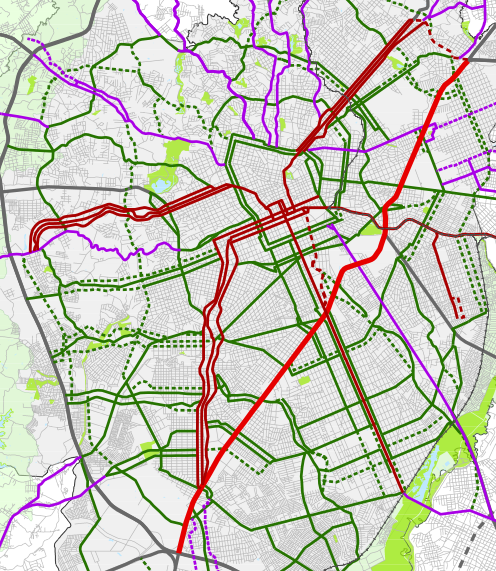
\includegraphics[width=0.5\textwidth]{fig/axes.png}
    \label{fig:axis}
    \par SOURCE: \textcite{Curitiba2015}.
\end{figure}

In addition, the Densification Axes acts as a complement to this urban structure, including a mixed land use and medium levels of density. Regarding the density, \textcite{Curitiba2015} establishes a low density as 80 residences per hectare, medium density between 80 and 200 residences per hectare and high density between 200 and 400 residences per hectare. \autoref{fig:macro} shows how these higher densities are set near the structural axes. Areas in red represent the higher density areas. 

\begin{figure}[!htbp]
    \centering\footnotesize
    \captionsetup{font=footnotesize}
    \caption{LAND USE DENSITIES IN CURITIBA}
    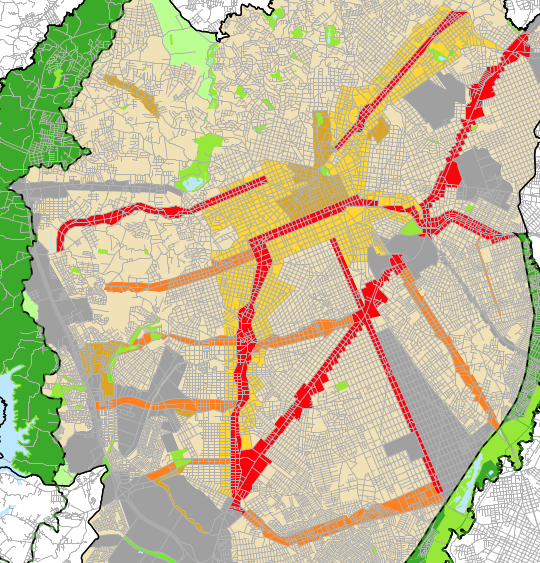
\includegraphics[width=0.6\textwidth]{fig/macro2.png}
    \label{fig:macro}
    \par SOURCE: \textcite{Curitiba2015}.
\end{figure}

Curitiba's land zoning plan splits the micro zoning system into four categories: central, residential, mixed use and specific destination \cite{Curitiba2019a}. Central zoning involves the traditional downtown of the city, characterized by a high concentration of services, commerces and jobs. Residential zones compasses different types, depending on the density. It can include commercial units and limited occupancy rate, depending on the environment characteristics. Mixed use zones encourages the coexistence of residential and non-residential uses, mixing residences, services and commercial units of medium density. Specific destination zoning can include educational, military, historic and industrial uses, among others. 

From decades ago until today, the majority of the urban environment was built for and around the needs of cards. Building and land use codes contribute to the causes of road traffic accidents, including speeding \cite{Knoflacher2016}. Cities and its decision makers needs to mind the traffic safety problems that are generated by the planning practices, as well the vantages of creating new spaces and land patterns that favors the safety inside the city. 

\section{NATURALISTIC DRIVING STUDIES} \label{nds}

Human behavior researches that focus on road traffic safety have multiple methods, including digital simulations, driving simulators and on-the-road studies. Digital simulations studies consists on the modelling of a hypothetical situation based on statistical and microssimulations functions which can be run multiple times on a software. Driving simulation studies contains a physical mockup of a real vehicle, where the subjects drives in accord to the computer-generated scenario. On-the-road studies consists of scenarios with real cars and traffic, and can be categorized into two types: experimental and observational studies \cite{Shinar2017}. 

\begin{figure}[!htbp]
    \centering\footnotesize
    \captionsetup{font=footnotesize}
    \caption{BEHAVIORAL TRAFFIC SAFETY STUDIES}
    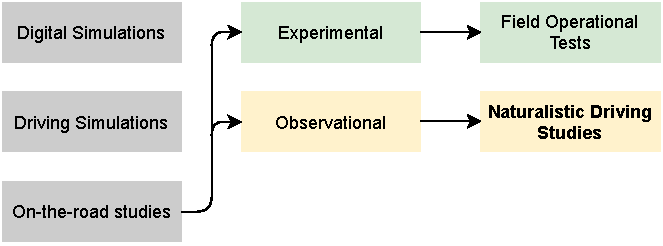
\includegraphics{fig/studies.pdf}
    \label{fig:shinar}
    \par SOURCE: The Author (2021), based on \textcite{Shinar2017}.
\end{figure}

Experimental studies contains some level of manipulation or control of the situation, where the independent variable is manipulated. This allows to better analyze the involved variables in a individual matter, but creates a artificial scenario, different from everyday situations. One popular type of experimental method is the field operational test (FOT). In FOT, volunteers are provided with cars equipped with multiple unobtrusive sensors, in order to investigate how they react to a specific system installed by the researchers. Diversely, observational studies simply observes the behavior of drivers in natural conditions, without the control of dependent and independent variables \cite{Shinar2017}. 

A type of observational study is the naturalistic driving study (NDS). NDS consists in monitoring drivers behavior in their own cars, both in normal and safety critical conditions. Volunteer's cars are usually equipped with video cameras, GPS systems and other sensors. The objective of the NDS is to record the driver's behavior during a everyday scenario. The cameras allows the recording of the driver, the car panel, instruments and the recording of the surrounding areas, including other vehicles, pedestrians and environmental elements. GPS or similar equipments allows register of the driver's instant speed and position \cite{Shinar2017}. Therefore, NDS is a method that can collect information about the environment, the vehicle and the human behavior.

The main difference between FOT and NDS is the element of study. FOT's usual objective is to evaluate a particular system or instrument inside or outside the vehicle. NDS' main objective is to record typical driving behaviors in multiple situations, including ones that presents a risk for the occurrence of road traffic crashes, like speeding occurence, use of mobile phones, etc. NDS generates a great number of data in comparison to other methods like FOT and driving simulators, but the method has its disadvantages as well. 

NDS in behavioral studies could be considered as an ``improvement'' in comparison to driving simulation studies, but its advantages and disadvantages makes them complementary methods, not competitive. In a driving simulation, the sample size is smaller, and the immersion is not perfect, given the possibility of the occurrence of motion sickness and adaptation period of the volunteers. But the main strength of driving simulators is the fact that it creates and controls the events and stimulus occurred in the scenario, making possible to better isolate variables and replicate crashes, near crashes and critical events \cite{Shinar2017}.   

In comparison, NDS have a typically large sample size and gives practically total immersion to the volunteers' everyday trips. The events occurred in traffic are totally uncontrolled and real. This gives a higher ``credibility'' to the data collected, but makes it harder to isolate the desired variables in study. The exposure to the experiment is usually higher in NDS, where the volunteers have the data registered over multiple trips \cite{Carsten2013}. Overall, the NDS characteristics and advantages are valuable to the present study, considering its capability of collecting a comparably large dataset of speeds and location throughout the city's territory.

\autoref{tab:nds} presents some of the main NDS researches that were established in the last two decades. The 100-Car Naturalistic Driving Study, conducted by the Virginia Tech Transportation Institute, was the first large scale NDS and was performed in the United States. Its instrumentation was composed of 5 cameras, 1 accelerometer and 1 GPS sensors, among others. Some of the vehicles were owned by the researchers and others by the volunteers. The main location of study was the metropolitan of northern virginia and Washington, DC. The main goal of the research was to maximize the potential to record crash and near-crash events. In total, 100 vehicles were used, with 241 drivers among primary and secondary volunteers. The total trip time of the data collected was above 40,000 hours, with a distance above 3 million kilometers \cite{Neale2005}.

\begin{table}[!hbtp]
    \footnotesize
    \captionsetup{justification=raggedright,
        singlelinecheck=false,
        font=footnotesize}
    \caption{NATURALISTIC DRIVING STUDIES PROGRAMS}
    \centering
    \begin{tabular}{llllll}
        \hline
        \multicolumn{1}{c}{\textbf{Program}} & \multicolumn{1}{c}{\textbf{Countries}} & \multicolumn{1}{c}{\textbf{Vehicles}} & \multicolumn{1}{c}{\textbf{Drivers}} & \multicolumn{1}{c}{\textbf{Hours}} & \multicolumn{1}{c}{\textbf{Distance} $[km]$} \\
        \hline
        100 Car NDS & USA & 100 & 241 & 42,300 & 3,218,688 \\
        SHRP2 NDS & USA & 3,500$^{(2)}$ & 3,500$^{(2)}$ & 1,000,000$^{(2)}$ & 56,327,040 \\
        ANDS & Australia & 346 & 409 & 716,320 & 1,512,630 \\
        UDRIVE & EU$^{(1)}$ & 192 & 287 & 87,870 & 4,000,000$^{(2)}$ \\
        CNDS & Canada & 140 & 149 & 53,000$^{(2)}$ & 1,800,000$^{(2)}$ \\ 
        \hline
    \end{tabular}
    \label{tab:nds}
    \par \vspace{2mm} \footnotesize \raggedright
    SOURCE: The Author (2021).
    \par \vspace{1mm} \footnotesize \raggedright
    NOTES: $^{(1)}$: UK, Netherlands, France, Spain, Germany and Poland; $^{(2)}$: Approximate values.
\end{table}

Another NDS study performed in the United States was the SHRP2 (Strategic Highway Research Program-2) NDS, gathering a massive quantity of data. The study was conducted in 6 states, with more than 3,500 vehicles, million hours of video and trip data collected and 56 million kilometers travelled among all the trips. More than 1,500 crashes were registered, establishing a valuable sample for road safety studies \cite{Njord2015}. The Australian Naturalistic Driving Study (ANDS) launched in 2015, aiming to collect road safety data from 360 vehicles - 180 in Sydney and 180 in Melbourne. The vehicles are equipped with 4 cameras, GPS sensors and accelerometer \cite{ANDS2017a}. Accordingly to \textcite{Larue2019}, the ANDS was able to collect data from 346 vehicles and 409 participants. The last report related a collection of more than 700,000 hours of travelled period and more than 1,500,000 kilometers of travelled distance \cite{ANDS2017a}. 

In the European Union, the UDRIVE naturalistic driving study was large scale NDS program installed in 6 EU countries: UK, Netherlands, France, Spain, Germany and Poland. It lasted for 5 years, between 2012 and 2017, and its objective was to collect behavioral data from three transport modes: cars, trucks and powered two-wheelers. 192 vehicles and 287 drivers were part of the research. The data collected reached almost 90,000 hours of driving data and approximately 4,000,000 kilometers of travelled distance \cite{VanNes2019}. The Canadian Naturalistic Driving Study (CNDS) instrumented a total of 140 vehicles, including cars, pickup trucks and minivans, with 4 cameras, a frontal radar sensor and one GPS radar. 149 drivers participated in the study, with approximately 53,000 hours of data collected amd 1,800,000 kilometers of travelled distance \cite{CNDS2021}. 

In Brazil, a naturalistic driving study was established in 2019 in the city of Curitiba-PR, conducted by the Universidade Federal do Paraná. The Naturalistic Driving Study - Brazil (NDS-BR) has already collect data from 16 instrumented vehicles, each with a kit of 3 cameras and 1 GPS sensor. Currently, NDS-BR collected almost 240 hours of driven time and 5,000 km of travelled distance in Curitiba and metropolitan area. This research its still ongoing, and further details about the process of data collection will be discussed in Section \ref{ndsc}. In all the previous NDS researches described, the collection of speed data was a possible due to the GPS sensors or accelerometers.


NDS allows the investigation of speeding episodes and how other factors can influence the occurence of speeding. These factors can include environmental elements (road infrastructure, built environment, weather, traffic conditions, etc.), human and behavior elements (age, gender, secondary tasks engagement, education, personality) and vehicle characteristics (engine power, level of conservation). \textcite{Richard2013,Richard2017, Richard2020} utilized NDS speed data to better understand different types of speeding and how the drivers behaves towards them. \textcite{Richard2013} established a classification called behavioral speeding, splitting it into 4 types. The first type consists of speed below the posted limit. In the second type, drivers are speeding but they feel like they are driving at a safe speed. On the third type, speeds reaches above the enforcement limit, where the driver starts to accept a higher level of risk. The 4th type consists of reckless speeding, where the driver reaches speeds way above the posted speed, without any consideration to the risks. 

\textcite{Richard2017} clustered speeding behavior into 6 categories, from a NDS data collected from 88 drivers in Seattle. The authors used the k-means method on the sample, resulting in 6 clusters: (i) Speeding up, (ii) speed drop, (iii) incidental speed, (iv) casual speeding, (v) cruising speeding and (vi) aggressive speeding. Speeding up behavior consists on reaching a high exceeding speed in a short period of time. with a high variability. Speed drop is complementary to speeding up, representing characteristics that are consistent with a braking behavior when entering a lower posted speed zone. 

Incidental speeding was the most common speeding type detected in the sample. It consists of mean speeds barely reaching above the posted speed, occurring in longer periods of time. Casual speeding was the second most common type, and has a similar behavior to incidental speeding, but has a higher level of mean speed above the posted speed, with similar lengths of occurrence. Cruising speeding is a deliberate type of speeding, most common on freeways and state highways - places with more opportunity for speeding. Aggressive speeding presents higher levels of mean speed, with a high variability in longer periods of time. In this cluster, drivers engages in repeated speed adjustments, always trying to reach maximum speed.

\textcite{Richard2020} used a sample of 100 trips from the SHRP2 NDS database in order to examine how the occurence of speeding episodes are affected by basic factors. The authors found drivers in the age group between 16 to 24 had more speeding episodes than other age categories. Considering the days of the week, the occurrence of speeding was lower between monday and thursday. Highways present higher free-flow and speeding episodes in comparison to other type of roads. 

\textcite{Ellison2015} analyzed speeding data from 106 drivers in Sydney, collected with the use of NDS, in order to establish how much time drivers are saving with speeding in urban environments. The speeding stretch of a trip was compared to a simulated stretch with the posted speed traveling the same length. Then, the time delta between the two scenarios was calculated to create the time saved during the speeding episode. The results showed a average time saving of 26 seconds per day, or 3 minutes per week. Considering the median driver, less than 2 hours per year is saved, and 75\% of drivers never save more than 3 min in a single day. 

\textcite{Hamzeie2017} investigated how the average speed chosen by drivers was influenced by the traffic conditions and how it affected the risk crashes. The authors used the SHRP2 NDS data and concluded that higher travel speeds were directly correlated to higher speed limits, and high speed variance is correlated to higher risk of crash. \textcite{Kong2020} also investigated speeding behavior patterns related to the traffic and road conditions, from a sample of naturalistic data collected from 92 vehicles. The authors concluded that speeding duration is related to driving on roadways with higher function classes, to longer trips and to speed loss causes by congestion, causing a idea of needing to ``recover the lost time'' by the drivers.

Using the BR-NDS data, \textcite{Bastos2021} compared traffic risks behavior between carpooling and non carpooling drivers, including speeding. The authors concluded that carpooling drivers presented a safer behavior towards speeding, having less episodes in comparison to non carpooling drivers. \textcite{Bastos2020a} also investigated the occurrence of mobile phone use (MPU) while driving and concluded that MPU occurs in higher frequencies when the average speed is lower. To analyze the relationship between speeding and speed cameras, \textcite{Amancio2021} also used the BR-NDS dataset. 

Overall, the papers cited in this Section are just a small sample of the existing studies including speeding behavior and NDS data. The NDS projects that were concluded or are ongoing generates an ample database of speeds and speeding episodes, making possible to continually investigate this risk behavior. 

\section{GEOGRAPHICALLY WEIGHTED REGRESSION} \label{sec:gwr}

Regression analysis is a tool to investigate the dependency between variables and to predict future parameters based on previous ones. This type of statistical analysis can show the relationship between dependent variables \cite{Lindley1987}. In investigation of the effects of the built environment on the occurrence of crashes in urban areas, negative binomial (NB) regression is a traditional model used \cite{Wei2013, Zhang2014}. But the quality of this model is limited by the incapacity of analyzing the spatial dependency and heterogeneity expected to happen on road safety factors related to the urban environment \cite{Obelheiro2019}.

% Explain better why GWR is batter and how the previous studies are less precise. 

To overcome this limitation, the Geographically Weighted Regression (GWR) allows the exploration of the relationship between variables on a spatial nonstationarity context. The spatial nonstationarity is a scenario where it is assumed that parameters are not constant across the space. A global regression model may be incapable of explaining the relationship between sets of variables with a acceptable level of precision in this scenario. The GWR model considers that the nature of the model must alter over space to reflect the structure within the data, allowing the actual parameters for each location in space to be modeled and mapped \cite{Brunsdon2010}.

The basic form of GWR, is based on the following equation:\begin{align}
    y_i = \beta_{i0} + \sum_{k=1}^{m} \beta_{ik} x_{ik} + \epsilon_i \mbox{;}
    \label{eq:gwr}
\end{align} where $y_i$ is the dependent variable at location $i$, $x_{ik}$ is the value of the $k$th independent variable at location $i$, $m$ is the number of independent variables, $\beta_{i0}$ is the intercept parameter at location $i$, $\beta_{ik}$ is the local regression coefficient for the $k$th parameter at location $i$ and $\epsilon_i$ is the random error at location $i$. The GWR model depends on a spatial weighting function called $w_{ij}$ that controls the contribution of the point $j$ on the calibration of a model for point $i$. The spatial weighting function represents the idea that for each point $i$ there is a bump of influence around it. Considering this "bump", observations closer to $i$ have more influence in the estimation of $i$'s parameters \cite{Brunsdon2010,Gollini2013}.

In the context of a multivariate GW model, these influences are calculated by a weighted least squares approach, described on the following equation: \begin{align}
    \hat{\beta}_i = \left(X^TW\left(u_i,v_i\right)X\right)^{-1}X^TW\left(u_i, v_i \right)y\mbox{ ;}
    \label{eq:wls}
\end{align} where $X$ is the matrix of the independent variables with a column of 1s (ones) for the intercept, $y$ is the dependent variable vector, $\hat{\beta} = \left(\beta_{i0},...,\beta_{im}\right)^T$ is the vector of $m + 1$ local regression coefficients and $W_i$ is the diagonal matrix denoting the spatial weighting ($w_{ij}$) of each observed data for regression point $i$ at location $(u_i, v_i)$ (defined by the selected spatial weighting function) \cite{Gollini2013}. The spatial weighting function is also known as the kernel function. This function can have multiple configurations, including Gaussian, Exponential, Boxcar, Bisquare and Tricube configurations, detailed on \autoref{tab:kernel}.

\begin{table}[!hbtp]
    \footnotesize
    \captionsetup{justification=raggedright,
        singlelinecheck=false,
        font=footnotesize}
    \caption{KERNEL FUNCTIONS}
    \centering
    \begin{tabular}{ll}
        \hline
        \multicolumn{1}{c}{\textbf{Kernel}} & \multicolumn{1}{c}{\textbf{Equation}}  \\
        \hline
        Global Model             & $w_{ij} = 1$                              \\
        Gaussian \rule{0pt}{3ex} & $w_{ij} = \exp \left(- \frac{1}{2} \left(\frac{d_{ij}}{b}\right)^2\right)$ \\
        Exponential  \rule{0pt}{4ex} & $w_{ij} = \exp \left(- \frac{|d_{ij}|}{b}\right)$               \\
        Boxcar \rule{0pt}{4ex} & $w_{ij} = \begin{cases}
            1 & \mbox{if } |d_{ij}| < b, \\
            0 & \mbox{otherwise}
                                 \end{cases}$                               \\
        Bisquare \rule{0pt}{4ex} & $w_{ij} = \begin{cases}
            \left(1 - \left(d_{ij}/b\right)^2\right)^2 & \mbox{if } |d_{ij}| < b, \\
            0 & \mbox{otherwise}
                                 \end{cases}$                               \\
        Tricube \rule{0pt}{4ex} & $w_{ij} = \begin{cases}
            \left(1 - \left(|d_{ij}|/b\right)^3\right)^3 & \mbox{if } |d_{ij}| < b, \\
            0 & \mbox{otherwise}
                                 \end{cases}$                               \\
        \hline
        \end{tabular}
    \label{tab:kernel}
    \par \vspace{2mm} \footnotesize \raggedright
    SOURCE: \textcite{Gollini2013}
\end{table}

The distance between observations $i$ and $j$ is defined by $d_{ij}$, inside a chosen $b$ bandwidth, which is the key controlling parameter in all kernel functions. \autoref{fig:kernel} presents the plot of the kernel functions, for a generic bandwidth $b = 1000$, where $w$ is the weight and $d$ is the distance between two observations. As the plot shows, the global kernel function represents a global linear regression, where all the variables are constant across the space. The bandwidth has two configurations: fixed or adaptive. Fixed bandwidth consists of a absolute value of distance, presenting better outcomes for uniform sized zonal levels \cite{Huang2018}, including grids with equal areas. Adaptive bandwidth consists in choosing a fixed quantity of neighbors for each regression point $i$, with variable sizes. This configuration works better for zonal levels with irregular sizes, including traffic analysis zones (TAZ) and census blocks \cite{Yu2017}. The size of bandwidth can be chosen with the use of a cross-validation function or testing multiple values to reach a lower value of corrected Akaike information criterion (AICc). These processes will be better explored in Section \ref{gwm}.

\begin{figure}[!htbp]
    \centering\footnotesize
    \captionsetup{font=footnotesize}
    \caption{KERNEL FUNCTIONS PLOT}
    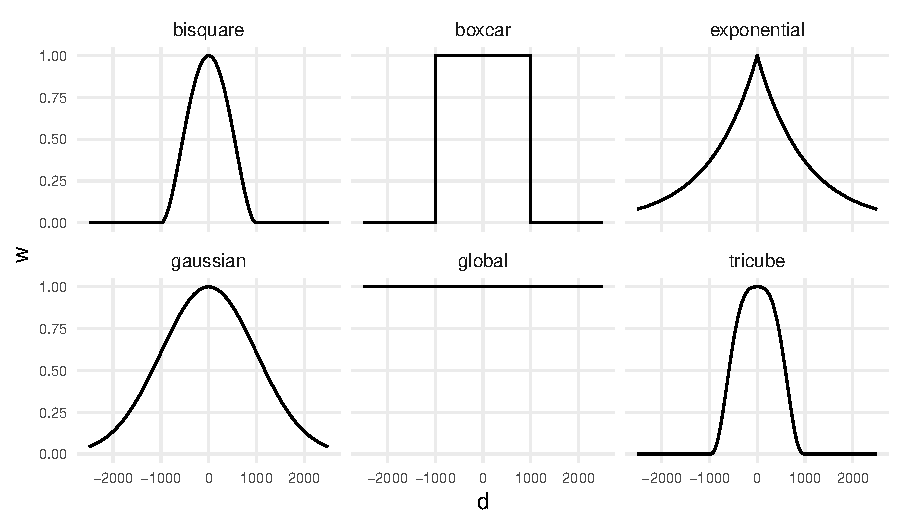
\includegraphics{fig/kernel.pdf}
    \label{fig:kernel}
    \par SOURCE: The Author (2021), based on \textcite{Gollini2013}.
\end{figure}

The GWR model presented on equation \ref{eq:gwr} has a limitation: it can be used only when the distribution of the dependent variable is Gaussian \cite{DaSilva2013a}. Therefore, count data needs other GWR configurations in order to fit in the model, including Poisson a Negative Binomial distributions. The Geographically Weighted Poisson Regression (GWPR) is described by \textcite{Obelheiro2020,Nakaya2005a} with the following equation: \begin{align}
    y_i \sim \mbox{ Poisson} \left[t_i \exp \left(\sum_k \beta_{ik} \left( u_{i}, v_{i} \right) x_{ik} \right) \right] \mbox{ ;}
\end{align} where $t_i$ is an offset variable and remaining variables are defined in equations \ref{eq:gwr} and \ref{eq:wls}. The Geographically Weighted Negative Binomial Regression (GWNBR) described by \textcite{DaSilva2013a} with the following equation: \begin{align}
    y_i \sim \mbox{ NB} \left[t_i \exp \left( \sum_k \beta_{ik} \left( u_{i}, v_{i} \right) x_{ik} \right), \alpha \left( u_{i}, v_{i}\right) \right] \mbox{ ;}
\end{align} where NB represents negative binomial and $\alpha$ is the parameter of overdispersion with spatial variation $\left(u_i, v_i\right)$. 

\autoref{tab:gwrworks} contains studies in which GWR models are used to investigate the relationship between BE variables and road safety performance, measured by the occurence of road crashes. In regard to zonal level, most investigations used TAZ as unit of analysis. \textcite{Obelheiro2020} created a traffic safety zonal level (TSAZ) based on census blocks. All authors but one used an area as zonal level. \textcite{Arvin2019} performed GWR models using intersection points as location of regression. 

\begin{table}[!htbp]
    \footnotesize
    \captionsetup{justification=raggedright,
        singlelinecheck=false,
        font=footnotesize}
    \caption{GWR AND ROAD SAFETY STUDIES}
    \centering
    \begin{tabular}{lllp{1.6cm}l}
        \hline
        \multicolumn{1}{c}{\textbf{Author}} & \multicolumn{1}{c}{\textbf{Zonal level}} & \multicolumn{1}{c}{\textbf{Distribution}} & \multicolumn{1}{c}{\textbf{Kernel}} & \multicolumn{1}{c}{\textbf{Bandwidth}} \\
        \hline 
        \textcite{Amoh-Gyimah2017} & TAZ, grid & Poisson & Bisquare, gaussian & Adaptive \\
        \textcite{Arvin2019} & Intersections & Poisson & Bisquare, gaussian & Adaptive \\
        \textcite{Hadayeghi2010} & TAZ & Poisson & Bisquare, gaussian & - \\
        \textcite{Huang2018} & Census block & Gaussian & - & Fixed \\
        \textcite{Obelheiro2019} & TAZ & Poisson, NB & - & Adaptive \\
        \textcite{Obelheiro2020} & TSAZ & Poisson, NB & - & Adaptive \\
        \textcite{Pirdavani2014} & TAZ & Gaussian & Bisquare, gaussian & Adaptive \\
        \textcite{Rhee2016} & TAZ & Gaussian & Gaussian & Fixed \\
        \textcite{Yu2017} & Census block & NB & - & Adaptive \\
        \textcite{Zhang2015} & TAZ & Poisson & - & - \\
        \hline
    \end{tabular}
    \label{tab:gwrworks}
    \par \vspace{2mm} \footnotesize \raggedright
    SOURCE: The Author (2021)
\end{table}

Regarding the type of GW model, most authors chose GWNBR or GWPR, considering that road crash count distribution fits better in these models. In relation to kernel type, it only varied between two options: Bisquare and Gaussian. Most studies contained the use of adaptive kernels, which is a better option for zonal level with irregular sizes. In conclusion, GWR is a method that enables the exploration of findings that might otherwise be missed if only a global regression method is applied. It is always important to really check if the GWR model will describe the data better than a global regression model comparing the results from both. All the process of constructing a GWR model and its parameters for this work is described in Section \ref{gwm}.

% ----------------------------------------------------------------------------------

\chapter{METHODS}

\section{THE BRAZILIAN NATURALISTIC DRIVING STUDY} \label{ndsc}

%% How data was collected, where it was collected, from who it as collected, when it was collected

%% Ref Jackson: gps2csv.py; functions.py; video.py ... (appendix)

% 1. Equipment: composition and how it was installed (equip. scheme - borguezani, camera scheme - amancio)

The Brazilian Naturalistic Driving Study (NDS-BR) utilized a non-intrusive instrumentation of vehicles, with two data acquisition system (DAS). Each DAS contains three high definition cameras, one GPS sensor, one laptop with a Linux distribution and one power supply. One camera was positioned on the right window of the car, towards the inside of the vehicle facing the driver. Two other cameras were positioned on the windshield of the car, facing towards the front outside. Considering these two, one camera is facing slightly to the left and another one to the right. The visual scheme of camera positioning is presented on \autoref{fig:cam_install}.

\begin{figure}[!htbp]
    \centering\footnotesize
    \captionsetup{font=footnotesize}
    \caption{CAMERA POSITIONING INSIDE THE VEHICLE}
    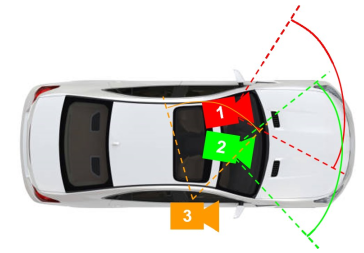
\includegraphics[width=0.6\textwidth]{fig/cam_install.png}
    \label{fig:cam_install}
    \par SOURCE: \textcite{Amancio2021}.
\end{figure}

The GPS sensor was positioned near the car panel. The cameras and GPS sensor were connected to the laptop, which controlled and synchronized the data acquisition. The laptop was installed inside a box, positioned on the floor by the passenger's seat. The DAS was installed in the personal vehicle of each volunteer. There was no audio collected from inside the vehicle, in order to not inhibit possible conversation of the driver during the study. Cameras 1 and 2 permitted the collection of visual data about the environment outside the vehicle - traffic conditions, traffic control, weather, conflicts with other vehicles, etc. Camera 3 permitted the collection of visual data about the behavior of the driver, including the use of seatbelt, mobile phone use, etc. \autoref{fig:cam_cap} shows images collected by the cameras.  

\begin{figure}[!htbp]
    \centering\footnotesize
    \captionsetup{font=footnotesize}
    \caption{CAMERA IMAGES}
    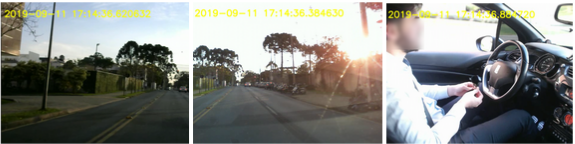
\includegraphics[width=0.9\textwidth]{fig/cam_cap.png}
    \label{fig:cam_cap}
    \par SOURCE: The Author (2021).
\end{figure}

% 2. Data processing: how they were processed (.py scripts), transformed to csv (gps2csv.py), valid time

The DAS kit allowed the acquisition of GPS and video data in synchronization, collecting information in a frequency of one second. The process of acquisition is illustrated in \autoref{fig:das}. The main controller of the data collection was the laptop. In the beginning of each trip, the driver needed to manually turn on the laptop after starting the car engine and before it started driving. A Bash script was written to run each time the laptop was turned on, with the objective to start two main Python scripts used in the data acquisition: gps-read.py and video.py \cite{Borguezani2020}.  

\begin{figure}[!htbp]
    \centering\footnotesize
    \captionsetup{font=footnotesize}
    \caption{NATURALISTIC DATA COLLECTION AND PROCESSING}
    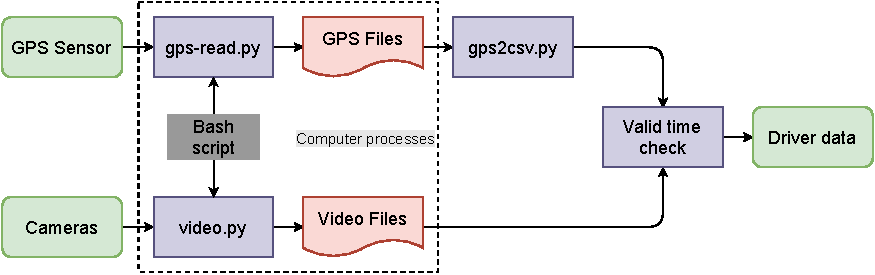
\includegraphics{fig/DAS.pdf}
    \label{fig:das}
    \par SOURCE: The Author (2021).
\end{figure}

The GPS sensor signals were translated into a .nmea format file, with the execution of gps-read.py. In order to analyze the collected data, after the NDS runs another Python script was used by the NDS-BR researchers to translate the .nmea into a .csv file. The GPS data contain information including latitude and longitude coordinates, date, time, speed, heading and altitude. The video files from all cameras were processed by the video.py script, having the timestamp and date printed on the screen. All the programs written in python are presented on Annex 1. 

After data was extracted from the laptop, it was necessary to make a valid time check, in order to exclude times from the final sample where the driver wasn't really driving the vehicle. \autoref{fig:validtime} presents how these invalid times where removed from the sample. For each trip, the period between the start of the car and when the volunteer started driving was considered as invalid. During the trip, if the driver pulled over briefly and then started driving again, this period between the actions was considered as invalid as well. Finally, the gap between parking the car and turning off the DAS was discarded from the sample.  

\begin{figure}[!htbp]
    \centering\footnotesize
    \captionsetup{font=footnotesize}
    \caption{VALID TIME SELECTION}
    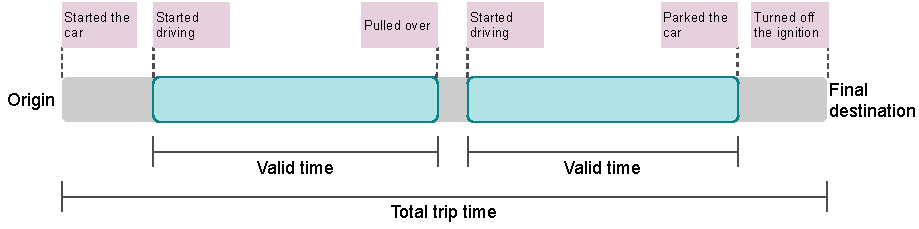
\includegraphics{fig/validtime.pdf}
    \label{fig:validtime}
    \par SOURCE: The Author (2021).
\end{figure}

The first trip of each driver was defined invalid. This trip was considered to be, to the driver, a time of getting familiar with the monitoring system. Moments with failure on the DAS, where the GPS or video data weren't properly recorded, also were considered as invalid time. The process of identifying invalid times was completely manual. A group of researchers identified the invalid times using the video data as reference. 

% 3. Drivers: How many, characteristics, data gathered, duration, how they were selected

The NDS-BR started collecting data on August, 2019. The local of the study is Curitiba and it's metropolitan region. Curitiba is the capital city of the State of Paraná, in Brazil. Until March of 2021, the project collected data from 16 volunteers, which composed the sample of naturalistic data used in this thesis. The drivers volunteered through a survey that was divulged in social networks. \autoref{tab:drivers} contains information about the participants and its vehicles, including the duration of data collection, age, gender, age of driver license, vehicle model year and horsepower.

\begin{table}[!htbp]
    \footnotesize
    \captionsetup{justification=raggedright,
        singlelinecheck=false,
        font=footnotesize}
    \caption{SELECTED PARTICIPANTS INFORMATION}
    \centering
    \begin{tabular}{lllllll}
        \hline
        \multicolumn{1}{c}{\textbf{ID}} & \multicolumn{1}{c}{\textbf{Duration}} & \multicolumn{1}{c}{\textbf{Age}} & \multicolumn{1}{c}{\textbf{Gender}} & \multicolumn{1}{c}{\textbf{License Age}} & \multicolumn{1}{c}{\textbf{Vehicle year}} & \multicolumn{1}{c}{\textbf{Horsepower}} \\
        \hline
        $D_1$ & 13 & 33 & F & 12 & 2012 & 96 \\
        $D_2$ & 12 & 40 & M & 3 & 2010 & 113 \\
        $D_3$ & 8 & 22 & M & 3 & 2011 & 103 \\
        $D_4$ & 16 & 25 & M & 6 & 2003 & 114 \\
        $D_5$ & 13 & 41 & F & 23 & 2014 & 75 \\
        $D_6$ & 13 & 28 & M & 9 & 2013 & 163 \\
        $D_7$ & 17 & 45 & M & 18 & 2011 & 130 \\
        $D_8$ & 12 & 32 & F & 10 & 2015 & 79 \\
        $D_9$ & 11 & 29 & M & 9 & 2019 & 74 \\
        $D_{10}$ & 14 & 62 & M & 37 & 2018 & 69 \\
        $D_{11}$ & 6 & 28 & F & 10 & 2012 & 75 \\
        $D_{12}$ & 5 & 45 & F & 26 & 2001 & 101 \\
        $D_{13}$ & 14 & 21 & F & 2 & 2006 & 81 \\
        $D_{14}$ & 6 & 34 & M & 16 & 2014 & 124 \\
        $D_{15}$ & 8 & 49 & F & 24 & 2018 & 84 \\
        $D_{16}$ & 11 & 27 & M & 3 & 2014 & 109 \\
        \hline
    \end{tabular}
    \label{tab:drivers}
    \par \vspace{2mm} \footnotesize \raggedright
    SOURCE: The Author (2021)
    \par \vspace{1mm} \footnotesize \raggedright
    NOTES: Duration in days; age and license age in years; M-male; F-female
\end{table}

The age of the drivers varied between 21 and 62 years old, with 7 females and 9 males. The duration of data collection from each driver varied between 5 and 17 days. Regarding the volunteers' vehicles, the model year varied between 2001 and 2019, with horsepower varying between 74 and 163 HP. All volunteers received a briefing on how to operate the equipment and signed a term of agreement, allowing the use of their data to academic research purposes. Overall, a total of 491 trips were made, resulting in 238.85 hours of driving and 5,362.75 km of distance travelled.

Only driver $D_{14}$ had a car with automatic gearbox. All other drivers had vehicles with a manual gearbox. Drivers $D_{1}$, $D_{2}$, $D_{3}$ e $D_{4}$ casually made trips in carpooling situation, offering rides to strangers with the use of carpooling apps. Drivers $D_{14}$, $D_{15}$ and $D_{16}$ worked as mobility app drivers. This caused a greater participation from them in the overall sample, which will be observed in the results.  

%% Start of NDS, how much time each collected

\section{DATA PROCESSING AND VARIABLE CONSTRUCTION} \label{data}

%% Data processing flowchart

This section includes the methods utilized to construct all the utilized variables, divided into two subsections: the speeding variable (dependent variable) and built environment variables (independent variables). \autoref{fig:methods} presents a brief flowchart on the process of transforming the data sources into a complete dataset included in the traffic analysis zones.  

\begin{figure}[!htbp]
    \centering\footnotesize
    \captionsetup{font=footnotesize}
    \caption{VARIABLE DATA FLOWCHART}
    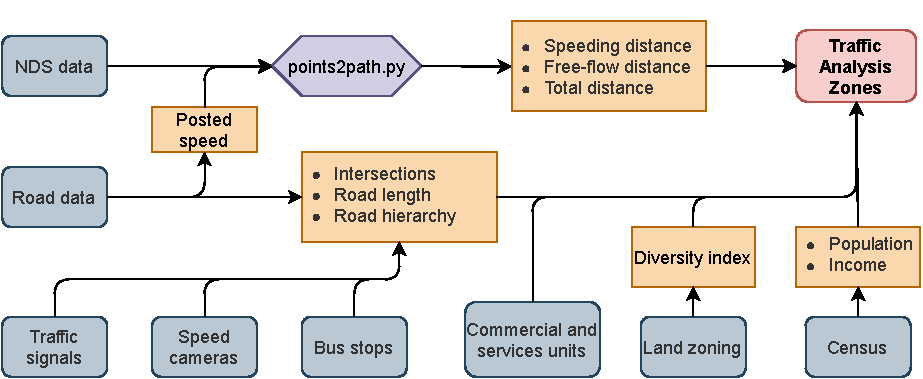
\includegraphics{fig/methods.pdf}
    \label{fig:methods}
    \par SOURCE: The Author (2021).
\end{figure}

\subsection{Speeding}

%% How speeding was measured (NSHTA)

%% How the main dataframe was constructed

% 1. Road axis buffer

% 2. Intersection with nds points

In order to extract speeding information from the NDS sample, it was necessary to compare the performed speeds from drivers with the respective posted speed. Posted speed data was collected from the road axis shape file obtained from OpenStreetMap \cite{OpenStreetMap}, completing some missing information with posted speeds from IPPUC road axis shape files \cite{IPPUC2021}. Using the software QGIS, it was created a 10 meter buffer around the road axes. In sequence, a intersection between the NDS points and the road buffer was performed, in order to associate the posted speed and the performed speed to the same point in space. This process is illustrated in \autoref{fig:buffer}. 

\begin{figure}[!htbp]
    \centering\footnotesize
    \captionsetup{font=footnotesize}
    \caption{ROAD AXIS BUFFER}
    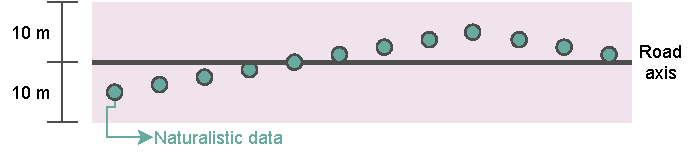
\includegraphics{fig/buffer.pdf}
    \label{fig:buffer}
    \par SOURCE: The Author (2021).
\end{figure}

Points with coordinates outside the buffers (in the middle of street blocks, for example) were removed from the sample. Also, points without posted speed and without performed speed data were removed from the sample. The extraction of free-flow and speeding events followed a method defined by \textcite{Richard2013}, presented in \autoref{fig:ff}. The occurence of speeding is represented by the proportion of distance travelled in speeds above the posted speed, divided by the distance performed in free-flow speeds. It is necessary to remove sections of the sample where drivers had no opportunity to speed. Therefore, the occurence of speeding is defined the following equation: \begin{align}
    SP = \frac{D_{Vsp}}{D_{Vf}} \mbox{ ;} 
\end{align} where $D_{Vsp}$ is the distance performed in speeds exceeding 5 km/h above the posted speed (analytical approach) and $D_{Vf}$ is the distance performed in free-flow speeds. Free-flow speeds includes performed speeds higher than the posted speed minus 10 km/h, and lower than speeding. \autoref{fig:spd_occur} presents a section of a trip, illustrating the thresholds previously described.   

% 3. Filtering points: speed exposure and speeding - explain criteria (based on richards)

\begin{figure}[!htbp]
    \centering\footnotesize
    \captionsetup{font=footnotesize}
    \caption{SPEEDING OCCURENCE AND SPEEDING OPPORTUNITY}
    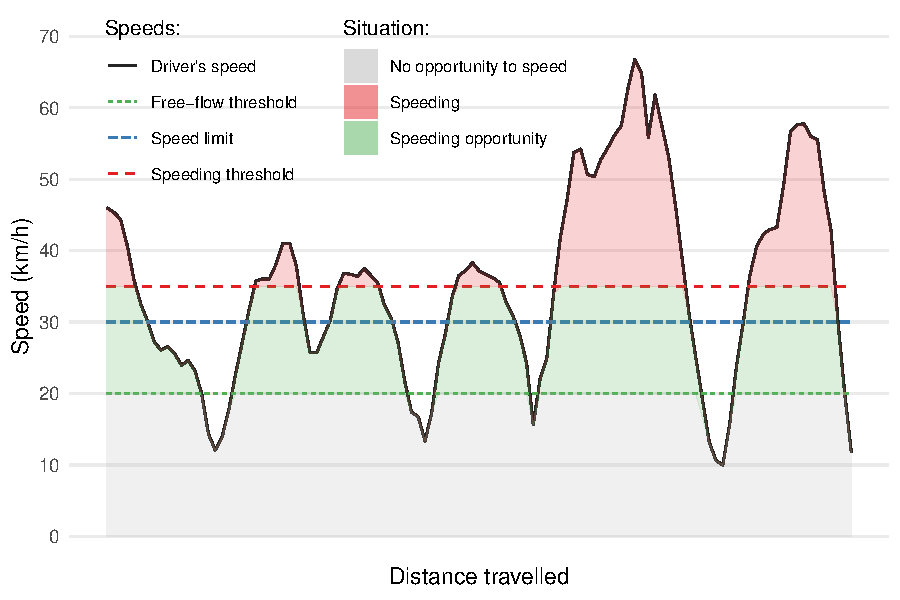
\includegraphics{fig/spd_occur.pdf}
    \label{fig:spd_occur}
    \par SOURCE: The Author (2021).
\end{figure}

% 4. transforming points into lines to export distances: linestring - python script

To extract distance data from the gps coordinates, it was made a conversion from the coordinates into a linestring, a geometry type from the Well-known text (WKT) format. QGIS is able to read the WKT format and calculate the distances. Only points with a 1 second gap from each other (observed from the time variable) were connected with a linestring. The conversion process was made with a python script, included on Appendix 1. Total distances, distances performed in free-flow speeds and distances in speeding were calculated for each TAZ in Curitiba, in order to calculate the occurence of speeding. 

\subsection{Built Environment}

%% How the independent variables were calculated

%% How the TAZ shape was constructed

% 1. TAZ shape (general info, source)

All variables (speeding and built environment) were calculated for each traffic analysis zone (TAZ) inside Curitiba. 135 TAZs, established in Curitiba's origin / destiny research made by IPPUC in 2018, were used for this work \cite{IPPUC2018b}. The BE variables that were calculated are listed in \autoref{tab:bivar}. Inside the density category, population data was obtained from the last Brazilian Census in 2010 \cite{IBGE2010}. Using the available census blocks, it was possible to calculate the population density (PD) data into the TAZs. 

% 2. Table with all variables: group & variable & abbreviation & unit & expected correlation to speeding

\begin{table}[!htbp]
    \footnotesize
    \captionsetup{justification=raggedright,
        singlelinecheck=false,
        font=footnotesize}
    \caption{BUILT ENVIRONMENT VARIABLES}
    \centering
    \begin{tabular}{lll}
        \hline
        \multicolumn{1}{c}{\textbf{Category}} & \multicolumn{1}{c}{\textbf{Variable}} & \multicolumn{1}{c}{\textbf{Description}} \\
        \hline
        Density & PD & Population Density [inhab/$km^2$]\\
        Diversity & LDI & Land use diversity index \\
        \multirow[t]{5}*{Design} & DIS & Density of intersections [no./km] \\
                              & DSC & Density of speed cameras [no./km] \\
                              & TSD & Traffic signal density [no./km] \\
                              & PAR & Proportion of arterial roads \\
                              & SND & Street network density [$km/km^2$] \\
        Destination accessibility & DCSU & Density of commercial and services units [no./$km^2$] \\
        Distance to transit & BSD & Bus stop density [no./km] \\
        Demographics & AVI & Average income [BRL] \\
        \hline
    \end{tabular}
    \label{tab:bivar}
    \par \vspace{2mm} \footnotesize \raggedright
    SOURCE: The Author (2021)
\end{table}

% 3. Independent variables calc (how each one was made) - Insert maps for each variable

Inside the diversity category, the land use diversity index (LDI) used information from Curitiba's zoning plan \cite{Curitiba2019a} as input for it's calculation. For each TAZ, the diversity index was calculated based on the following equation \cite{Huang2018}:\begin{align}
    LDI = \frac{-\sum_i^n P_i \times \ln(P_i)}{\ln(n)} \mbox{ ;}
\end{align} where $i$ is the type of land use, $n$ is the total number of land use types in a TAZ and $P_i$ is the proportional area of land use type $i$. LDI varies between 0 and 1, where 0 represents a single land use zone and 1 represents a perfect distribution of land uses. The GIS data of each zoning type was obtained from \textcite{IPPUC2021}. PD and LDI variables are plotted in \autoref{fig:pd_ldi}.

\begin{figure}[!htbp]
    \centering\footnotesize
    \captionsetup{font=footnotesize}
    \caption{PD AND LDI}
    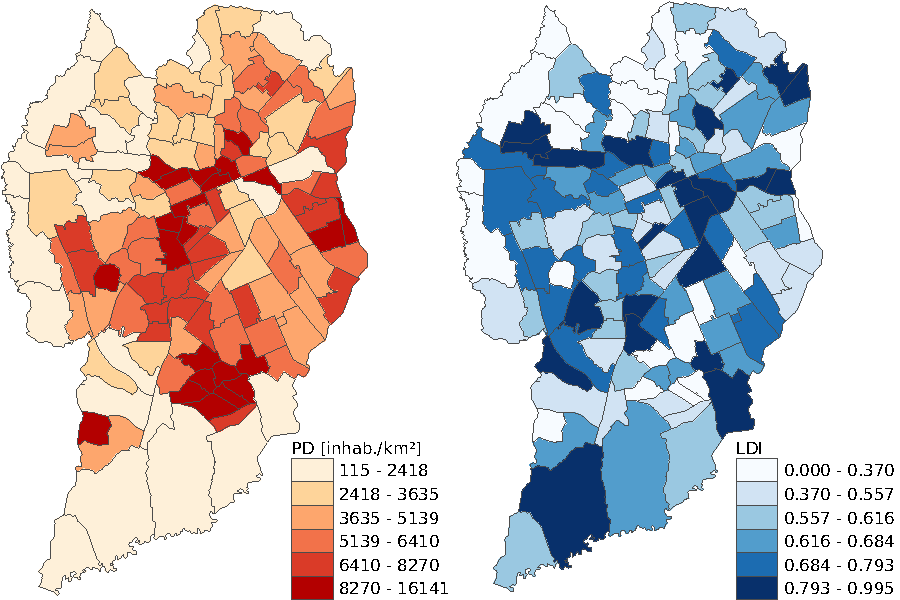
\includegraphics{fig/map_PD+LDI.pdf}
    \label{fig:pd_ldi}
    \par SOURCE: The Author (2021), based on \textcite{IBGE2010, IPPUC2018b, IPPUC2021}.
\end{figure}

In regard to the design category, the density of intersections (DIS) was calculated based on the number of intersections divided by the length of roads. The intersection points and road lengths were extracted from the \textcite{IPPUC2021} road axis data. Intersection points were extracted using the "line intersection" function included in QGIS. Density of speed cameras (DSC) and traffic signal density (TSD) follows the same method applied on density of intersections. Speed camera points were obtained from the Municipal Office of Social Defense and Transit of Curitiba \cite{SETRAN2020} and traffic signal points were obtained from \textcite{IPPUC2021}. DIS and DSC variables are plotted in \autoref{fig:dis_dsc}. 

\begin{figure}[!htbp]
    \centering\footnotesize
    \captionsetup{font=footnotesize}
    \caption{DIS AND DSC}
    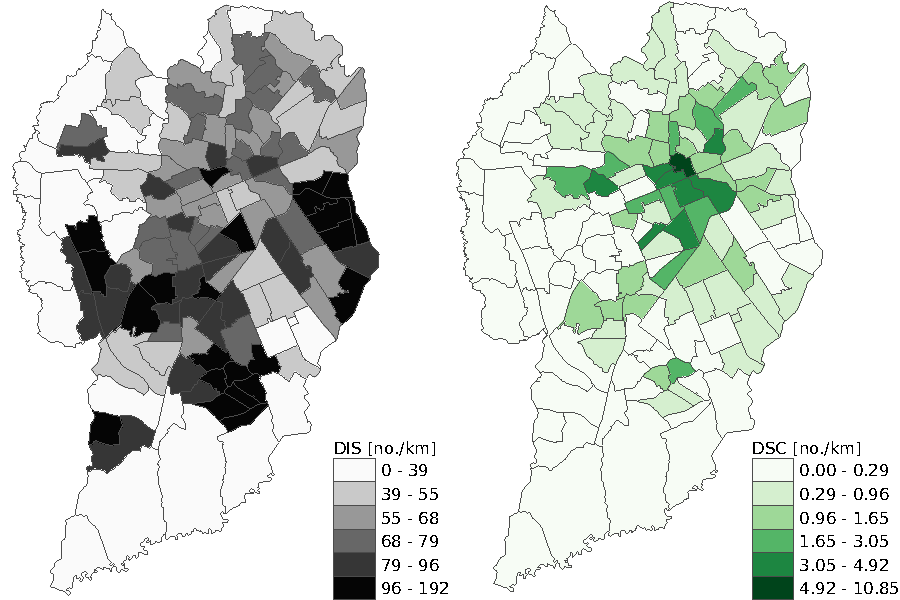
\includegraphics{fig/map_DIS+DSC.pdf}
    \label{fig:dis_dsc}
    \par SOURCE: The Author (2021), based on \textcite{IPPUC2018b,IPPUC2021,SETRAN2020}
\end{figure}

The proportion of arterials (PAR) used the IPPUC road axis data as well. The road hierarchy data follows the categories established by the Brazilian Traffic Code \cite{Brasil1997}: Rapid transit, arterial, collector and local roads. In this variable, rapid transit and arterial roads were combined into one category representing arterial roads. Hence, the proportion of arterial roads was based on the division between arterial roads length and total road length. TSD and PAR variables are plotted in \autoref{fig:tsd_par}

\begin{figure}[!htbp]
    \centering\footnotesize
    \captionsetup{font=footnotesize}
    \caption{TSD AND PAR}
    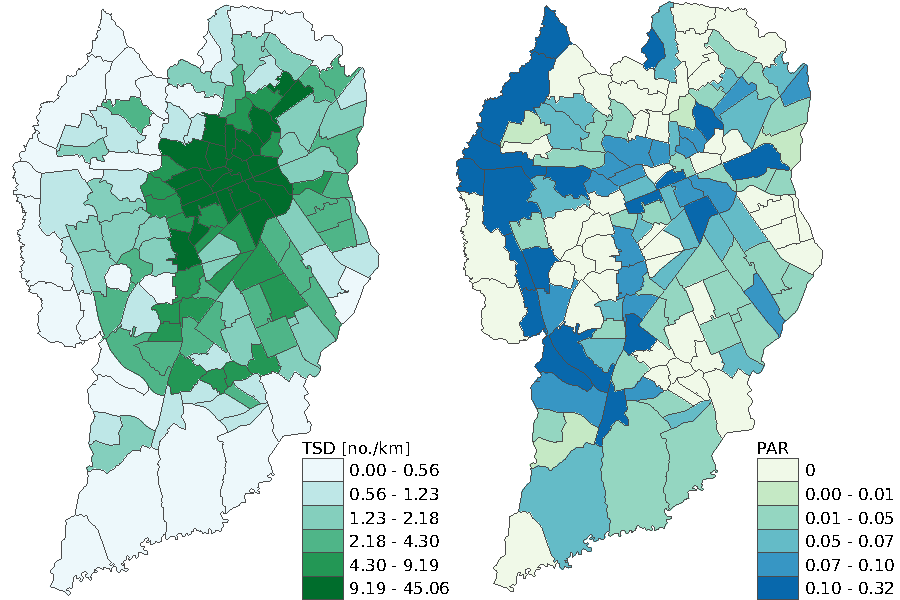
\includegraphics{fig/map_TSD+PAR.pdf}
    \label{fig:tsd_par}
    \par SOURCE: The Author (2021), based on \textcite{IPPUC2018b,IPPUC2021}
\end{figure}

Street network density (SND) is the total road length divided by the area in squared kilometers of the respective TAZ. Regarding the destination accessibility, the location of commercial and services units from 2019 was provided by \textcite{IPPUC2021}, making possible the calculation of the density of commercial and services units (DCSU) per TAZ. SND and DCSU variables are plotted in \autoref{fig:snd_dcsu}.

\begin{figure}[!htbp]
    \centering\footnotesize
    \captionsetup{font=footnotesize}
    \caption{SND AND DCSU}
    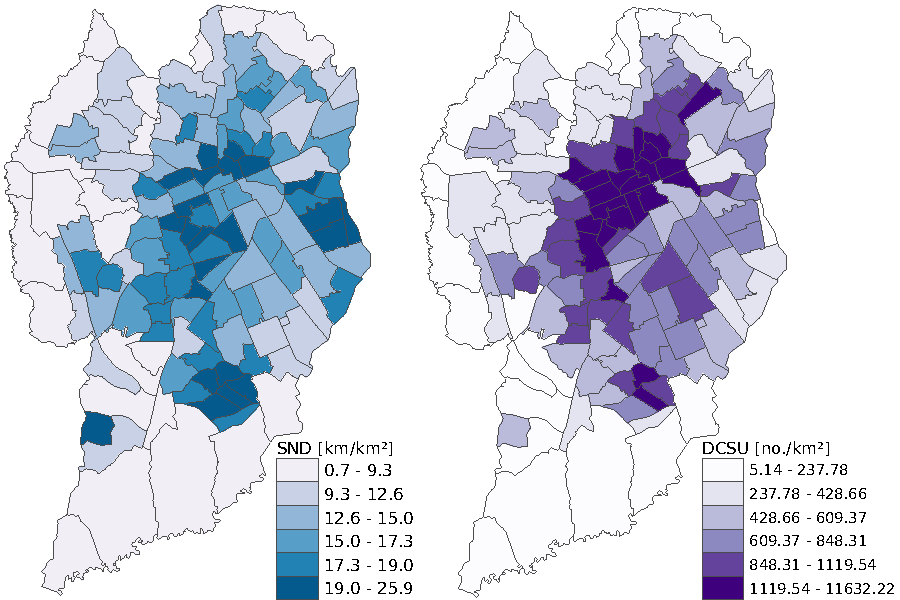
\includegraphics{fig/map_SND+DCSU.pdf}
    \label{fig:snd_dcsu}
    \par SOURCE: The Author (2021), based on \textcite{IPPUC2018b,IPPUC2021}
\end{figure}

The distance to transit is represented by the bus stop density (BSD) per road length. The location of bus stops across the city was provided by \textcite{IPPUC2020a}, with data from 2020. The average income (AVI), representing the demographics category, was obtained from the Brazilian Census of 2010 \cite{IBGE2010}. BSD and AVI variables are plotted in \autoref{fig:bsd_avi}. 

\begin{figure}[!htbp]
    \centering\footnotesize
    \captionsetup{font=footnotesize}
    \caption{BSD AND AVI}
    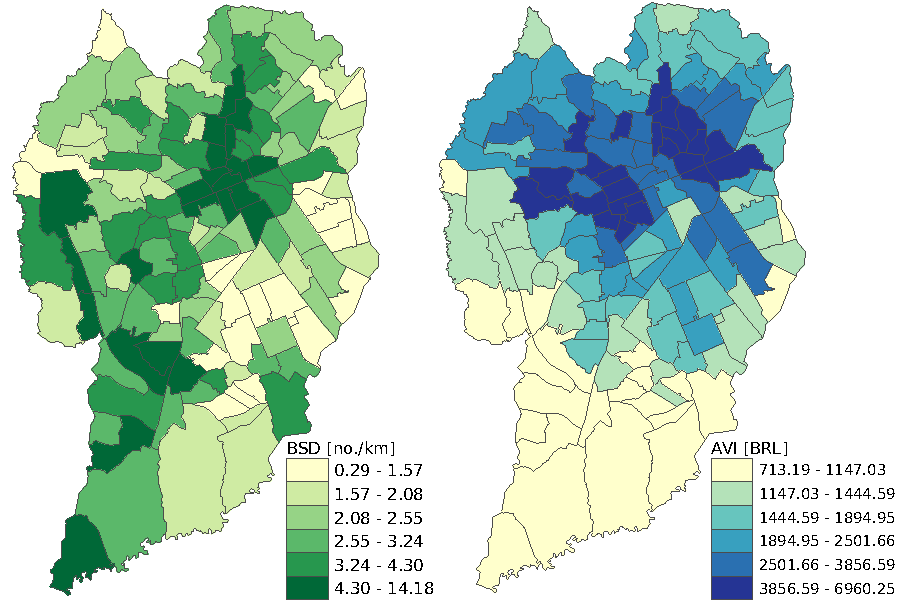
\includegraphics{fig/map_BSD+AVI.pdf}
    \label{fig:bsd_avi}
    \par SOURCE: The Author (2021), based on \textcite{IPPUC2018b,IPPUC2020a, IBGE2010}
\end{figure}

\section{GEOGRAPHICALLY WEIGHTED REGRESSION MODELLING} \label{gwm}

%% How the model was constructed: Inputs, outputs

%% Describe each possible config (NB, poisson, GLM)

%% Performance measures (AICc, global R-squared, Morans I on residuals)

%% What each function does on code

%% basically a walk through of the code (ref code on appendix)

% ----------------------------------------------------------------------------------

\chapter{ANALYSIS AND RESULTS}

% 1. Results from NDS (how much each driver participated)

%% How much each driver participated: Quantity of trips, length of trips (mean, median, 1q, 3q, max , min) - try table or boxplot

\begin{table}[!htbp]
    \footnotesize
    \captionsetup{justification=raggedright,
        singlelinecheck=false,
        font=footnotesize}
    \caption{TRIP DISTANCES RESULTS}
    \centering
    \begin{tabular}{lrrrrrrrrr}
        \hline
        \multicolumn{1}{c}{\textbf{Driver}} & \multicolumn{1}{c}{\textbf{n}} & \multicolumn{1}{c}{\textbf{Mean}} & \multicolumn{1}{c}{\textbf{SD}} & \multicolumn{1}{c}{\textbf{Min.}} & \multicolumn{1}{c}{\textbf{1Q}} & \multicolumn{1}{c}{\textbf{Median}} & \multicolumn{1}{c}{\textbf{3Q}} & \multicolumn{1}{c}{\textbf{Max.}} & \multicolumn{1}{c}{\textbf{Total distance}} \\ 
        \hline
        $D_{1}$ & 29 & 5.49 & 2.36 & 1.17 & 4.70 & 5.84 & 6.13 & 12.60 & 159.33 \\ 
        $D_{2}$ & 14 & 14.09 & 7.81 & 2.41 & 7.14 & 14.40 & 21.94 & 22.70 & 197.31 \\ 
        $D_{3}$ & 15 & 11.58 & 4.41 & 4.16 & 7.89 & 11.86 & 14.82 & 19.14 & 173.72 \\ 
        $D_{4}$ & 48 & 4.26 & 2.47 & 0.24 & 2.30 & 3.50 & 5.88 & 9.36 & 204.67 \\ 
        $D_{5}$ & 56 & 2.71 & 2.86 & 0.00 & 0.66 & 2.14 & 3.72 & 15.69 & 152.01 \\ 
        $D_{6}$ & 37 & 3.21 & 1.44 & 0.90 & 1.99 & 2.82 & 4.45 & 6.85 & 118.83 \\ 
        $D_{7}$ & 29 & 10.84 & 5.60 & 0.48 & 5.12 & 12.88 & 15.67 & 17.04 & 314.44 \\ 
        $D_{8}$ & 31 & 6.40 & 3.55 & 0.67 & 2.46 & 7.00 & 9.15 & 13.14 & 198.55 \\ 
        $D_{9}$ & 11 & 4.63 & 2.04 & 1.69 & 3.24 & 4.51 & 5.87 & 7.63 & 50.92 \\ 
        $D_{10}$ & 40 & 5.65 & 4.02 & 0.41 & 2.04 & 5.05 & 8.80 & 14.87 & 225.97 \\ 
        $D_{11}$ & 12 & 1.72 & 1.63 & 0.17 & 0.66 & 1.07 & 2.30 & 5.90 & 20.62 \\ 
        $D_{12}$ &  6 & 1.71 & 2.38 & 0.07 & 0.21 & 0.46 & 2.51 & 5.97 & 10.28 \\ 
        $D_{13}$ & 23 & 3.97 & 2.01 & 0.10 & 2.96 & 3.94 & 4.94 & 7.51 & 91.26 \\ 
        $D_{14}$ & 31 & 21.06 & 17.28 & 0.06 & 7.70 & 17.68 & 30.05 & 72.93 & 652.71 \\ 
        $D_{15}$ & 21 & 38.33 & 40.40 & 1.33 & 10.73 & 25.57 & 47.75 & 168.26 & 805.02 \\ 
        $D_{16}$ &  7 & 12.04 & 15.21 & 0.02 & 3.69 & 3.92 & 14.99 & 42.97 & 84.27 \\ 
        \hline
    \end{tabular}
    \label{tab:trips}
    \par \vspace{2mm} \footnotesize \raggedright
    SOURCE: The Author (2021)
    \par \vspace{1mm} \footnotesize \raggedright
    NOTES: Distances in kilometers. 
\end{table}


%% hour of the day, day of the week (per distance travelled, per number of trips)

%% how much travelled in each TAZ (MAP)

% 2. Speeding Results

%% how much speeding for each driver (per trip - mean, median, 1q, 3q, max, min - try table AND boxplot) 

\begin{table}[!htbp]
    \footnotesize
    \captionsetup{justification=raggedright,
        singlelinecheck=false,
        font=footnotesize}
    \caption{SPEEDING PER TRIP RESULTS}
    \centering
    \begin{tabular}{lrrrrrrr}
        \hline
        \multicolumn{1}{c}{\textbf{Driver}} & \multicolumn{1}{c}{\textbf{Mean}} & \multicolumn{1}{c}{\textbf{SD}} & \multicolumn{1}{c}{\textbf{Min.}} & \multicolumn{1}{c}{\textbf{1Q}} & \multicolumn{1}{c}{\textbf{Median}} & \multicolumn{1}{c}{\textbf{3Q}} & \multicolumn{1}{c}{\textbf{Max.}} \\
        \hline
        $D_1$ & 0.29 & 0.17 & 0.07 & 0.16 & 0.27 & 0.39 & 0.63 \\ 
        $D_2$ & 0.35 & 0.16 & 0.09 & 0.20 & 0.43 & 0.47 & 0.53 \\ 
        $D_3$ & 0.48 & 0.17 & 0.23 & 0.32 & 0.48 & 0.60 & 0.78 \\ 
        $D_4$ & 0.32 & 0.14 & 0.00 & 0.26 & 0.31 & 0.40 & 0.66 \\ 
        $D_5$ & 0.25 & 0.24 & 0.00 & 0.03 & 0.18 & 0.40 & 0.79 \\ 
        $D_6$ & 0.48 & 0.15 & 0.10 & 0.39 & 0.47 & 0.59 & 0.74 \\ 
        $D_7$ & 0.26 & 0.14 & 0.03 & 0.18 & 0.25 & 0.33 & 0.76 \\ 
        $D_8$ & 0.33 & 0.21 & 0.00 & 0.18 & 0.26 & 0.52 & 0.70 \\ 
        $D_9$ & 0.46 & 0.13 & 0.23 & 0.37 & 0.49 & 0.58 & 0.62 \\ 
        $D_{10}$ & 0.35 & 0.22 & 0.00 & 0.17 & 0.35 & 0.46 & 0.79 \\ 
        $D_{11}$ & 0.26 & 0.19 & 0.00 & 0.13 & 0.28 & 0.36 & 0.64 \\ 
        $D_{12}$ & 0.30 & 0.30 & 0.00 & 0.04 & 0.27 & 0.47 & 0.76 \\ 
        $D_{13}$ & 0.26 & 0.18 & 0.00 & 0.15 & 0.22 & 0.34 & 0.79 \\ 
        $D_{14}$ & 0.46 & 0.17 & 0.00 & 0.40 & 0.49 & 0.58 & 0.79 \\ 
        $D_{15}$ & 0.38 & 0.12 & 0.07 & 0.33 & 0.39 & 0.47 & 0.57 \\ 
        $D_{16}$ & 0.56 & 0.19 & 0.30 & 0.45 & 0.57 & 0.70 & 0.79 \\ 
        \hline 
    \end{tabular}
    \label{tab:speeding}
    \par \vspace{2mm} \footnotesize \raggedright
    SOURCE: The Author (2021).
\end{table}


%% How much speeding in each TAZ (map)

%% hour of the day, day of the week (per distance travelled, per number of trips)

%% How much each driver made speeding (hour of the day, day of the week)

%% NSHTA diagram of speeding (talvezzzz)

% 3. Results from GWR

%% Summary of variables: mean, median, max, min, 1q, 3q

%% Show models results (quality variables) - AICc, morans I, R-squared

%% Chosen model based on results

%% Map and discuss the variables

% ----------------------------------------------------------------------------------

\chapter{CONCLUSIONS}
